\documentclass[11pt]{report}
\usepackage[T1]{fontenc}
\usepackage[utf8]{inputenc}
\usepackage{textcomp}
\usepackage[margin=1in]{geometry}
\usepackage{booktabs}
\usepackage{graphicx}
\usepackage{hyperref}
\usepackage{xcolor}
\usepackage{verbatim}
\usepackage{amsmath}
\usepackage{amssymb}
\usepackage{siunitx}
\usepackage{multirow}

\newcommand{\code}[1]{\texttt{\small #1}}
\hypersetup{colorlinks=true, linkcolor=blue, citecolor=blue, urlcolor=blue}

\title{Multimodal AAD dataset --- analysis progress}
\author{OSU / PAS2301}
\date{\today}

\begin{document}
\maketitle
\tableofcontents
\clearpage

\chapter*{Dataset layout}
\addcontentsline{toc}{chapter}{Dataset layout}

For every subject, two data stores hold parallel copies of the same trials,
partitioned by modality.

\section*{\code{experiment\_data/Subject N/}}
\begin{itemize}
  \item \code{Training-1} \ldots \code{Training-5} --- 5 familiarisation trials
        at the start of the recording session.
  \item \code{Eval-1} \ldots \code{Eval-100} --- 100 main trials.
        \code{Eval-K} corresponds to the \code{Trial-K} row of
        \code{audio\_stimuli\_data/trials.csv}.
  \item Each trial folder holds EEG (\code{eeg\_data.p}, 32-ch @ \SI{500}{\Hz})
        and \code{audio\_timestamps.json}.
\end{itemize}

\section*{\code{Video Recordings/Subject N/}}
Per-subject folders numbered \code{1} through \code{105}:
\begin{itemize}
  \item Folders \code{1}--\code{5} = training trials (same ordering as
        \code{experiment\_data/Training-K}).
  \item Folders \code{6}--\code{105} = main trials; folder \code{K}
        corresponds to \code{Eval-(K-5)} (i.e.\ \code{Trial-(K-5)}).
  \item Each folder holds the Tobii Glasses~3 bundle:
        \code{gazedata.gz} (per-eye gaze direction + pupil + scene-projected
        gaze), \code{imudata.gz}, \code{scenevideo.mp4},
        \code{eventdata.gz}, \code{recording.g3}, \code{snap0.jpg}.
\end{itemize}

Subjects 1 and 2 use literal numeric folder names (\code{1}\ldots\code{105}).
Subjects 3--16 use ISO-8601 timestamps (\code{YYYYMMDDTHHMMSSZ}); the loader
parses the embedded time and sorts ascending to recover the natural recording
order. This ordering is verified empirically against audio playback
timestamps to $r_\Delta \geq 0.99$ trial-to-trial for every subject.

\section*{Gaze source}
The authoritative gaze stream is the Tobii \code{gazedata.gz} inside each
Video-Recordings folder (per-eye 3-D gaze direction, pupil diameter,
scene-projected \code{gaze2d}, 3-D \code{gaze3d}). Experiment-data 2-D gaze
files are not used in the current pipeline.

\section*{Audio}
\code{audio\_stimuli\_data/trials.csv} lists per-trial metadata:
attended-speaker index, the three device files, SNR in dB, and per-channel
powers. Speech files live in \code{audio\_stimuli\_data/pairs/*.flac} as
stereo; each device plays one stereo file with its two channels driving
the two speakers of that device.

\subsection*{Speaker geometry (listener-referenced azimuth)}
\begin{center}
\begin{tabular}{lrll}
\toprule
Label & Azimuth & Device / channel & Hemisphere \\
\midrule
1 & $-67.5^\circ$ & Device-1 Left  & LEFT \\
2 & $-22.5^\circ$ & Device-1 Right & LEFT \\
3 & $+22.5^\circ$ & Device-2 Left  & RIGHT \\
4 & $+67.5^\circ$ & Device-2 Right & RIGHT \\
-- & $-135^\circ$ & Device-3 Left  (noise) & back \\
-- & $+135^\circ$ & Device-3 Right (noise) & back \\
\bottomrule
\end{tabular}
\end{center}

Device-1 is the entire \textbf{left} hemisphere speaker pair; Device-2 is
the entire \textbf{right} hemisphere pair. Device-3 carries back-hemisphere
noise. All speakers are at a radial distance of \SI{4}{ft}.

\chapter{Analysis pipeline}
\label{ch:pipeline}

\section{Shared preprocessing}

\begin{itemize}
  \item EEG is loaded from \code{eeg\_data.p} (32\,ch, \SI{500}{\Hz}) and the
        32 scalp channels are wrapped in an \code{mne.io.Raw} with the
        ANT~Neuro 10--20 montage (Fp1, Fpz, Fp2, F7, F3, Fz, F4, F8, FC5,
        FC1, FC2, FC6, M1, T7, C3, Cz, C4, T8, M2, CP5, CP1, CP2, CP6, P7,
        P3, Pz, P4, P8, POz, O1, Oz, O2).
  \item \textbf{Bad-channel detection} flags flat channels
        (\code{std} < \num{1e-9}), saturated channels ($\geq 10\%$ samples at
        the \num{0.0839} ADC clip), and AC-variance $|z| > 6$ outliers
        against the median MAD of the remaining channels.
  \item \textbf{Referencing} defaults to linked mastoids (average of
        M1 and M2); when either mastoid is flagged bad, falls back to a
        common-average reference over the good channels. Flagged channels
        are then interpolated via spherical splines so every trial ends with
        32 valid channels.
  \item Notch filter at \SI{60}{\Hz}, band-pass 1--9\,Hz for speech-tracking
        analyses, and a subsequent resample to 64\,Hz (common rate with
        audio envelopes).
  \item Optional ICA with automatic EOG-component identification using
        Fp1/Fp2 as proxies (disabled by default because ablations showed
        only a \num{0.3}\,pp gain at $3\times$ runtime cost).
\end{itemize}

\section{Modality alignment}

All streams are clipped to the shared audio-playback window
$[t_0, t_1]$ derived from the per-trial \code{audio\_timestamps.json}:

\begin{itemize}
  \item \textbf{EEG}: internal \code{eeg\_ts} is mapped to wall-clock unix
        time via \code{first\_sample\_time} in \code{eeg\_time\_data.p}.
  \item \textbf{Tobii streams} (gaze + IMU): recording-relative timestamps
        are shifted so the first sample aligns to $t_0$, then clipped to
        $[t_0, t_1]$.
  \item \textbf{Audio envelopes}: computed from each device's stimulus file
        and re-sampled to match the EEG rate.
\end{itemize}

\section{EEG linear-decoder backbones (iter-3 on all 16 subjects)}

For each (subject $\times$ backbone) combination the pipeline:
\begin{enumerate}
  \item Loads 100 main trials, preprocessed as above at 64\,Hz.
  \item Builds lagged regressors over $[-200, +500]\,\text{ms}$ (step 25\,ms).
  \item Selects ridge $\alpha$ via an inner 5-fold CV on a 12-point
        log-spaced grid $10^{-1}\ldots10^6$, scored by mean
        $\rho_\text{att}-\rho_\text{una}$ on held-out trials.
  \item Outer 5-fold CV for reported accuracy at decision windows
        \{1, 2, 4, 8, 16, 30\,s\}.
\end{enumerate}

Four backbones:
\begin{itemize}
  \item \textbf{Broadband}: 1--9\,Hz Hilbert envelope derivative (half-wave
        rectified) as the 1-D reconstruction target.
  \item \textbf{Split $\delta$+$\theta$}: concatenated 1--4\,Hz and 4--8\,Hz
        EEG lag features, reconstructing the same 1-D envelope.
  \item \textbf{Mel-28}: 28-band gammatone-proxy mel envelope as the
        multi-band reconstruction target (reduced to mean-band for the
        scalar ridge).
  \item \textbf{CCA mel-28}: canonical correlation between (EEG lags) and
        (mel-28 envelope), retaining up to 5 components per trial.
\end{itemize}

\section{Multimodal fusion}

Binary group-level task: attended speaker pair $\in \{\text{Device-1},
\text{Device-2}\}$ (chance = 0.5). For each subject we compute:
\begin{itemize}
  \item \textbf{Gaze features} from the Tobii \code{gazedata.gz} stream ---
        mean/std of scene-projected gaze, per-eye gaze-direction azimuth
        and elevation, pupil diameter, saccade rate, 3-D gaze centroid,
        and IMU head motion.
  \item \textbf{EEG features} = the $(\rho_\text{att}, \rho_\text{una})$
        pair from each EEG backbone, mapped through a sigmoid to a
        per-trial probability.
\end{itemize}
Classifiers: logistic regression (gaze-only, EEG-only) and LightGBM
(stacked / early-fusion). Evaluated with 5-fold stratified CV per subject.

\section{SLURM design}

Account: \code{PAS2966}. Array jobs on the \code{batch} partition, one task
per (subject $\times$ backbone). Each task: 8 CPUs, 32\,GB memory, 2\,h wall
limit. A single backbone sweep across 16 subjects occupies 16 tasks;
iter-3's four backbones $=$ 64 tasks total, parallelised across compute
nodes so the full sweep wall-clocks in roughly 15--20 minutes.

\chapter{Current results}
\label{ch:results}

\section*{What task is being decoded}

\textbf{Goal}: for every trial (30\,s of concurrent multi-talker speech),
predict which of 4 spatial speakers (Device-1 L at $-67.5°$, Device-1 R
at $-22.5°$, Device-2 L at $+22.5°$, Device-2 R at $+67.5°$) the subject
was attending. Ground truth is the \code{Attended Speaker} column of
\code{trials.csv}.

\textbf{Evaluation}: 5-fold stratified CV \emph{per subject} over 100
main trials; accuracies are mean across folds. Pooled accuracy is the
unweighted mean of per-subject accuracies across all 16 subjects
(bootstrap 95\,\% CI).

\textbf{Inputs used in this chapter}:
\begin{itemize}
  \item \emph{Linear EEG decoder}: 32-ch EEG ($\sim$\SI{500}{\Hz})
        bandpassed to 1--9\,Hz and resampled to \SI{64}{\Hz}; decoder is
        CCA between EEG-lags ($-200\ldots+500$\,ms) and the 28-band
        gammatone envelope of the attended-device stereo audio
        (\emph{inputs: EEG only}; audio envelopes are the supervision
        signal, not classifier inputs).
  \item \emph{Fusion}: Tobii \code{gazedata.gz} per-trial summary
        (20 features) combined with the EEG CCA probabilities.
  \item IMU and scene video are not used in this chapter.
\end{itemize}

All 16 subjects, 100 main trials each. Within-subject 5-fold CV, 30\,s
full-trial decision windows unless stated otherwise.

\section{Linear EEG decoder (backward TRF / CCA)}

\subsection{Pooled full-trial accuracy (chance $= 0.5$)}

\begin{table}[ht]
\centering
\begin{tabular}{lrr}
\toprule
Backbone & Pooled mean & $n$ trials \\
\midrule
\textbf{CCA mel-28}              & \textbf{0.523} & 1599 \\
Mel-28 ridge                     & 0.511 & 1599 \\
Broadband ridge                  & 0.507 & 1599 \\
Split $\delta$+$\theta$          & 0.492 & 1599 \\
\midrule
Oracle adaptive (per-subject best backbone) & 0.555 & 1599 \\
\bottomrule
\end{tabular}
\end{table}

CCA on the 28-band gammatone envelope is the best uniform backbone. A
per-subject adaptive policy that picks whichever backbone wins on inner CV
reaches 0.555, $\sim 3$\,pp above the best fixed choice.

\subsection{Per-subject winning backbone}

\begin{table}[ht]
\centering
\begin{tabular}{ll}
\toprule
Backbone & Subjects for which it wins \\
\midrule
CCA mel-28              & S1, S2, S4, S5, S7, S10, S11, S12, S13 (9) \\
Broadband ridge         & S3, S9, S14, S16 (4) \\
Mel-28 ridge            & S6, S15 (2) \\
Split $\delta$+$\theta$ & S8 (1) \\
\bottomrule
\end{tabular}
\end{table}

\subsection{Window-length sweep (mean across 16 subjects)}

\begin{table}[ht]
\centering
\begin{tabular}{rrrr}
\toprule
Window (s) & Broadband & Mel-28 & Split $\delta$+$\theta$ \\
\midrule
1          & 0.496     & 0.499  & 0.500 \\
2          & 0.499     & 0.501  & 0.498 \\
4          & 0.500     & 0.505  & 0.499 \\
8          & 0.505     & 0.500  & 0.502 \\
16         & 0.510     & \textbf{0.524} & 0.504 \\
30         & 0.507     & 0.510  & 0.492 \\
\bottomrule
\end{tabular}
\end{table}

The short-window (1--4\,s) regime stays near chance; accuracy climbs
modestly at 16--30\,s. This shallow gradient reflects the 30\,s trial length
and the reduced stimulus separability of the paradigm (each device plays
one speech file across both of its L/R speakers at different powers, so
the attended and unattended streams are spatially smeared).

\section{Multimodal fusion}

Three task framings share the same Tobii-gaze feature set
(\code{gazedata.gz}) and the same EEG backbones, evaluated per subject via
5-fold stratified CV.

\subsection{Task A --- Attended hemisphere (left vs right)}

Binary task: attended speaker $\in$ Left hemisphere (labels 1--2, azimuth
$\{-67.5^\circ,-22.5^\circ\}$) vs Right hemisphere (labels 3--4, azimuth
$\{+22.5^\circ,+67.5^\circ\}$). Chance $= 0.5$.

\subsection{Pooled accuracy (bootstrap 95\,\% CI, $n = 16$)}

\begin{table}[ht]
\centering
\begin{tabular}{lcccccc}
\toprule
EEG backbone & Gaze-only & EEG-only (LR) & Late fusion & Stacked & Early fusion \\
\midrule
Broadband          & 0.770 & 0.505 & 0.766 & 0.752 & 0.751 \\
Split $\delta$+$\theta$ & 0.770 & 0.485 & 0.767 & 0.734 & 0.757 \\
Mel-28             & 0.770 & 0.511 & 0.756 & 0.758 & 0.763 \\
\textbf{CCA mel-28} & \textbf{0.770} & 0.502 & \textbf{0.768} & 0.756 & 0.764 \\
\bottomrule
\end{tabular}
\end{table}

Pooled 95\,\% CI for gaze-only: $[0.685, 0.849]$. EEG-only sits at chance on
the binary group-level task; fusion gives the same pooled number as
gaze-only within CI overlap.

\subsection{Per-subject attended-hemisphere AAD (CCA mel-28 backbone)}

\begin{table}[ht]
\centering
\begin{tabular}{lrrrrrr}
\toprule
Subj & $n$ & Gaze & EEG (LR) & Late & Stacked & Early \\
\midrule
1  &  99 & 0.404 & 0.545 & 0.394 & 0.545 & 0.515 \\
2  &  98 & 0.939 & 0.429 & 0.939 & 0.918 & 0.949 \\
3  & 100 & \textbf{1.000} & 0.340 & 0.990 & 0.990 & \textbf{1.000} \\
4  & 100 & 0.980 & 0.490 & 0.990 & 0.970 & 0.950 \\
5  & 100 & 0.750 & 0.520 & 0.730 & 0.710 & 0.750 \\
6  & 100 & 0.640 & 0.390 & 0.650 & 0.650 & 0.670 \\
7  & 100 & 0.910 & 0.420 & 0.900 & 0.920 & 0.930 \\
8  & 100 & 0.550 & 0.560 & 0.550 & 0.570 & 0.570 \\
9  & 100 & 0.660 & 0.560 & 0.680 & 0.620 & 0.670 \\
10 & 100 & 0.860 & 0.480 & 0.860 & 0.820 & 0.780 \\
11 & 100 & 0.680 & 0.570 & 0.680 & 0.610 & 0.610 \\
12 & 100 & 0.600 & 0.510 & 0.580 & 0.490 & 0.590 \\
13 & 100 & 0.860 & 0.630 & 0.840 & 0.850 & 0.890 \\
14 & 100 & 0.650 & 0.580 & 0.650 & 0.700 & 0.620 \\
15 &  99 & 0.980 & 0.556 & 0.980 & 0.980 & \textbf{1.000} \\
16 & 100 & 0.830 & 0.470 & 0.820 & 0.790 & 0.800 \\
\bottomrule
\end{tabular}
\end{table}

\subsection{Task B --- Inner vs Outer (gaze-lateralisation control)}

Binary task: inner speakers (labels 2, 3, azimuth $\pm 22.5^\circ$) vs
outer speakers (labels 1, 4, azimuth $\pm 67.5^\circ$). This collapses the
left/right axis and asks whether gaze can distinguish eccentricity. Pooled
gaze-only accuracy $= \mathbf{0.690}$ (vs 0.500 chance; 13/16 above
chance). A secondary spatial signal is present but substantially weaker
than the hemisphere task.

\subsection{Task C --- 4-class speaker identity}

4-way classification over the full speaker set (chance $= 0.25$). Pooled
accuracy $= \mathbf{0.547}$, 16/16 subjects above chance. Effect size
relative to chance ($+30$\,pp) is comparable to Task A's $+27$\,pp --- the
binary hemisphere task just happens to have a higher absolute chance.

\section{Observations}

\begin{enumerate}
  \item \textbf{Gaze carries the dominant signal for the attended
        hemisphere (Task A)}: 6/16 subjects reach $\geq 0.83$ gaze-only
        accuracy; S3 and S15 reach \textbf{1.000} with early fusion. Gaze
        is substantially weaker on within-hemisphere distinctions (Task
        B: 0.690 pooled).
  \item \textbf{Linear EEG-only AAD on the binary hemisphere task is at
        chance.} The backward TRF / CCA extracts per-trial
        envelope-tracking correlation, not a lateralised spatial
        signature --- so collapsing four speakers into two hemispheres
        loses the signal the decoder is most sensitive to.
  \item \textbf{Fusion does not yet improve pooled accuracy} because the
        EEG contribution is near-chance. The pipeline is wired end-to-end
        and ready to benefit from a stronger EEG model.
  \item \textbf{Per-subject heterogeneity is informative}. The five
        subjects below $0.70$ gaze-only (S1, S6, S8, S11, S12) are the
        ones whose gaze does not reliably fixate the attended source. These
        are the subjects for whom a non-gaze decoder is actually useful.
  \item \textbf{Subject 1} is an outlier: below-chance gaze (0.40) and
        near-chance EEG. The recording has 100\,\% flat M1 and 100\,\%
        saturated M2 --- a real hardware/electrode issue, not an analysis
        artefact. It survives the pipeline only because the robust
        referencing and spherical interpolation prevent the bad channels
        from corrupting the other 30.
\end{enumerate}

\chapter{Iteration 4 --- results}
\label{ch:iter4}

\section*{Task and inputs}

Same AAD task as Chapter~\ref{ch:results}: predict the attended speaker
from 30-s trials. Three experiments here, each varying \emph{only} the
EEG/gaze source or decoder architecture:

\begin{itemize}
  \item \textbf{4-class EEG decoder} (§\ref{sec:iter4-4class}): input =
        32-ch EEG at \SI{64}{\Hz}; supervision = 4 candidate attended
        envelopes (one per speaker). Target = pick the speaker. Gaze,
        IMU, and video are not used.
  \item \textbf{EEG$\leftrightarrow$gaze predictability}
        (§\ref{sec:iter4-pred}): input = 32-ch EEG (for EEG$\to$gaze) or
        the 20-D Tobii gaze summary (for gaze$\to$attended). Target =
        gaze time-courses, or the attended-speaker label.
  \item \textbf{Gaze-residualised EEG AAD}
        (§\ref{sec:iter4-resid}): input = 32-ch EEG \emph{after}
        channel-wise regression of a 15-feature Tobii gaze + IMU
        regressor set; same CCA-mel-28 decoder as Chapter~\ref{ch:results}
        otherwise. Target = attended-speaker hemisphere.
\end{itemize}

Per-subject 5-fold CV; pooled = unweighted mean across 16 subjects with
bootstrap 95\,\% CI. All 48 SLURM tasks completed on the
\code{PAS2966} CPU queue.

\section{4-class EEG speaker-identity decoder}
\label{sec:iter4-4class}

CCA between EEG lags ($-200\ldots+500$\,ms) and 28-band gammatone envelopes
of each of the 4 possible attended speakers (Device-1 L/R, Device-2 L/R).
Test trials are classified by \emph{argmax} canonical correlation across
the four envelope candidates. Per-subject 5-fold CV, 100 trials.

\subsection{Per-subject accuracy}

\begin{table}[ht]
\centering
\begin{tabular}{lrrr}
\toprule
Subject & 4-class & hemisphere & inner/outer \\
\midrule
1  & 0.240 & 0.490 & 0.480 \\
2  & 0.270 & 0.520 & 0.480 \\
3  & 0.260 & 0.430 & 0.610 \\
4  & 0.220 & 0.480 & 0.450 \\
5  & 0.310 & 0.560 & 0.520 \\
6  & 0.240 & 0.560 & 0.500 \\
7  & 0.330 & 0.500 & 0.610 \\
8  & 0.250 & 0.520 & 0.500 \\
9  & 0.250 & 0.490 & 0.540 \\
10 & 0.280 & 0.450 & 0.550 \\
11 & 0.250 & 0.500 & 0.550 \\
12 & 0.210 & 0.540 & 0.450 \\
13 & 0.230 & 0.450 & 0.510 \\
14 & 0.210 & 0.450 & 0.480 \\
15 & 0.263 & 0.505 & 0.545 \\
16 & 0.270 & 0.530 & 0.520 \\
\midrule
\textbf{Pooled} & \textbf{0.255}    & \textbf{0.498}    & \textbf{0.518} \\
95\,\% CI       & [0.240, 0.271] & [0.479, 0.517] & [0.496, 0.542] \\
Chance          & 0.250             & 0.500             & 0.500 \\
\bottomrule
\end{tabular}
\end{table}

All three task framings land at chance. The 4-class decoder does not
distinguish individual speakers; even the inner-outer binary barely
exceeds chance ($+1.8$\,pp). This is expected: within a device, the
stereo speech file is replicated on both channels with different
amplitudes --- the envelope shape is near-identical, so envelope
reconstruction cannot pick between the two channels of the same device.

Window sweep $\{1,2,4,8,16,30\}$\,s shows no gradient beyond
$\pm 0.01$, confirming the backbone is not merely data-starved.

\section{Cross-modal predictability (EEG $\leftrightarrow$ gaze)}
\label{sec:iter4-pred}

\subsection{EEG $\rightarrow$ gaze (ridge regression, held-out Pearson $r$)}

\begin{table}[ht]
\centering
\begin{tabular}{lrr}
\toprule
Target & mean $r$ & std \\
\midrule
gaze2d\_x (scene-projected horizontal) & \textbf{0.028} & 0.020 \\
gaze2d\_y (scene-projected vertical)   & 0.016 & 0.015 \\
gaze3d\_x (listener-ref horizontal, mm) & 0.009 & 0.011 \\
gaze3d\_y (vertical, mm)                & 0.000 & 0.012 \\
gaze3d\_z (depth, mm)                   & 0.002 & 0.008 \\
\bottomrule
\end{tabular}
\end{table}

EEG carries almost no linear predictive information about instantaneous
gaze: held-out Pearson $r$ peaks at $0.028$ for the horizontal
scene-projected gaze and collapses to zero in 3-D body-referenced space.

\subsection{CCA EEG $\leftrightarrow$ gaze (first-component correlation)}

\begin{table}[ht]
\centering
\begin{tabular}{lr}
\toprule
 & Mean first-component $r$ \\
\midrule
In-sample (training residuals) & 0.147 $\pm$ 0.092 \\
Held-out                        & \textbf{0.081} $\pm$ 0.063 \\
\bottomrule
\end{tabular}
\end{table}

A small but consistent shared subspace exists (held-out $r$ $= 0.081$),
but it is an order of magnitude below what each modality exposes about
the attended-speaker label on its own.

\subsection{Gaze $\rightarrow$ attended (logistic classifier)}

\begin{table}[ht]
\centering
\begin{tabular}{lrrr}
\toprule
Task              & Chance & Pooled & 95\,\% CI \\
\midrule
Hemisphere (L vs R) & 0.500 & \textbf{0.769} & [0.684, 0.851] \\
Inner vs outer      & 0.500 & 0.680          & [0.603, 0.762] \\
4-class identity    & 0.250 & 0.551          & [0.439, 0.668] \\
\bottomrule
\end{tabular}
\end{table}

Reproduces the corrected-mapping numbers from Chapter~\ref{ch:results}.

\section{Gaze-residualised EEG AAD --- the headline control}
\label{sec:iter4-resid}

For every trial, a 15-feature gaze/IMU regressor set
(\code{gaze2d\_x/y}, \code{gaze3d\_x/y/z}, per-eye direction, pupil
diameters, gaze velocities, \mbox{$|\text{accel}|{-}g$}, $|\text{gyro}|$)
is channel-wise ridge-regressed out of the EEG ($\lambda {=} 10^{-3}$)
\emph{before} the CCA mel-28 decoder sees it. Compares against the same
decoder on un-residualised EEG (\emph{baseline}). Per-subject 5-fold CV,
hemisphere task, full 30-s trial.

\begin{table}[ht]
\centering
\begin{tabular}{lrr}
\toprule
Subject & Baseline & Gaze-residualised \\
\midrule
1  & 0.560 & 0.580 \\
2  & 0.570 & 0.610 \\
3  & 0.380 & 0.460 \\
4  & 0.490 & 0.520 \\
5  & 0.510 & 0.570 \\
6  & 0.510 & 0.580 \\
7  & 0.580 & 0.580 \\
8  & 0.490 & 0.570 \\
9  & 0.560 & 0.560 \\
10 & 0.520 & 0.430 \\
11 & 0.510 & 0.530 \\
12 & 0.440 & 0.520 \\
13 & 0.510 & 0.590 \\
14 & 0.520 & 0.450 \\
15 & 0.424 & 0.505 \\
16 & 0.470 & 0.440 \\
\midrule
\textbf{Pooled}    & \textbf{0.503}    & \textbf{0.531} \\
95\,\% CI          & [0.477, 0.528]    & [0.503, 0.558] \\
\bottomrule
\end{tabular}
\end{table}

\noindent
Mean paired $\Delta = +0.028$\,pp. Wilcoxon signed-rank
$p = 0.084$, $n = 16$. 11 of 16 subjects improve after removing the
gaze-correlated variance.

\textbf{Headline result}: removing gaze-correlated variance from EEG
\emph{improves} AAD accuracy, not reduces it. This directly refutes the
``eye-tracking-in-disguise'' concern: EEG carries AAD-relevant signal
that is independent of gaze, and the gaze-linked component is
effectively noise relative to the TRF task.

\section{Extended fusion (gaze + 4-class-EEG-probabilities)}

Fusion inputs: Tobii gaze summary features (20-D) $+$ the 4-class CCA
softmax probabilities ($\text{p}_1, \ldots, \text{p}_4$). Classifier =
LightGBM ($n=200$ estimators) with 5-fold stratified CV per subject.
Three task framings; S15's 4-class EEG cache was missing so fusion is
computed on 15 subjects; gaze-only is pooled on all 16.

\begin{table}[ht]
\centering
\begin{tabular}{lrrr}
\toprule
Task              & Gaze-only & EEG-only (4-class probs) & Early fusion \\
\midrule
Hemisphere    & \textbf{0.770} & 0.501 & 0.749 \\
Inner vs outer & 0.690          & 0.477 & 0.643 \\
4-class identity & 0.547        & 0.255 & 0.493 \\
\bottomrule
\end{tabular}
\end{table}

\begin{itemize}
  \item Fusion does not exceed gaze-only on any task --- the 4-class EEG
        probabilities are too close to chance to add discriminative
        signal on top of a strong gaze feature vector.
  \item The \emph{only} bounded gain from fusion will come from either
        (a) a stronger EEG decoder (iter-5: deep models) or (b) subjects
        whose gaze is unreliable, where the EEG residual is additive.
  \item Per-subject fusion outperforms gaze-only only for 4 subjects
        on hemisphere task (S5: $+0.02$, S6: $+0.07$, S7: $+0.02$, S12:
        $+0.00$). These are the low-gaze-accuracy subjects --- exactly
        the regime where EEG is expected to help.
\end{itemize}

\section{What iter-4 settles}

\begin{enumerate}
  \item \textbf{Linear EEG alone cannot discriminate within-device L/R}
        (4-class $= 0.255$, chance $= 0.250$). The paradigm's stereo
        device design means envelope reconstruction is blind to channel
        identity. Iter-5 will test whether a deep decoder on
        \emph{raw EEG} (not reconstruction) can exploit the spatial
        lateralisation cues that CCA misses.
  \item \textbf{EEG has very low linear predictability of gaze}
        ($r \leq 0.03$) and a modest shared subspace
        ($r_\text{CCA, out} = 0.081$). Gaze contamination of EEG exists
        but is small.
  \item \textbf{Removing gaze \emph{improves} EEG-AAD by $+2.8$\,pp} ---
        the reviewer-ready answer to the ``eye-tracking in disguise''
        question.
  \item \textbf{The fusion story} needs a better EEG backbone to beat
        the gaze ceiling. The wiring is in place; iter-5 just swaps the
        EEG module.
\end{enumerate}

\chapter{Iteration 5 --- classical spectral EEG features}
\label{ch:iter5}

\section{Task definition and inputs}

\paragraph{Task.} Auditory-attention decoding: for a given trial, predict
which of four concurrently presented speakers the subject was attending
to. A trial is 30\,s long; during it the subject hears four speech
streams simultaneously (Device-1 L, Device-1 R, Device-2 L, Device-2 R
--- see Dataset Layout chapter) plus noise from Device-3 at ±135°. The
attended-speaker label comes from \code{trials.csv} and is one of
$\{1, 2, 3, 4\}$.

\paragraph{Three label-collapses evaluated.}
\begin{itemize}
  \item \textbf{Hemisphere} (chance $= 0.5$): $\{1,2\}$ (LEFT,
        az $\in\{-67.5°, -22.5°\}$) vs $\{3,4\}$ (RIGHT, az $\in\{+22.5°,
        +67.5°\}$). This is the classical binary AAD framing --- which
        side is the listener attending.
  \item \textbf{Inner vs outer} (chance $= 0.5$): $\{2,3\}$ (inner
        speakers at $\pm 22.5°$) vs $\{1,4\}$ (outer speakers at
        $\pm 67.5°$). Tests whether the decoder picks up \emph{eccentricity}
        rather than hemisphere.
  \item \textbf{4-class speaker identity} (chance $= 0.25$): predict the
        exact speaker label $1/2/3/4$.
\end{itemize}

\paragraph{Inputs used in iter-5.}
\begin{itemize}
  \item \textbf{EEG-only condition}: 32-channel EEG
        (\code{experiment\_data/Eval-K/eeg\_data.p}), bandpassed 1--40\,Hz,
        notched at 60\,Hz, auto-referenced (linked mastoids when good;
        common-average otherwise), at the native \SI{500}{\Hz}. Per trial
        we compute a \textbf{368-dimensional spectral feature vector}
        described in the next section and use it as input $X$ to a
        per-subject classifier.
  \item \textbf{Gaze-only condition} (for the fusion comparison): the
        Tobii Glasses~3 \code{gazedata.gz} stream from the Video-Recordings
        folder paired with the trial, plus the paired \code{imudata.gz}.
        The 30-s stream is summarised into a 23-dimensional vector
        (Table~\ref{tab:gaze-feats}). The experiment-data 2-D gaze
        (\code{gaze\_data.p}) is not used.
\end{itemize}

\begin{table}[ht]
\centering
\caption{Gaze / head-motion feature vector (23 features per trial).}
\label{tab:gaze-feats}
\begin{tabular}{llll}
\toprule
\# & Name & Source & Description \\
\midrule
1  & \code{gx\_mean}      & Tobii gaze2d & scene horizontal gaze, mean \\
2  & \code{gx\_std}       & Tobii gaze2d & scene horizontal gaze, std \\
3  & \code{gy\_mean}      & Tobii gaze2d & scene vertical gaze, mean \\
4  & \code{gy\_std}       & Tobii gaze2d & scene vertical gaze, std \\
5  & \code{gx\_valid}     & Tobii gaze2d & fraction of finite samples \\
6  & \code{sacc\_rate}    & derived       & saccades/s (I-VT, 30°/s thresh.) \\
7  & \code{sacc\_amp\_med} & derived      & median saccade amplitude (°) \\
8  & \code{g3d\_x\_mean}  & Tobii gaze3d & 3-D gaze x (horizontal, mm) \\
9  & \code{g3d\_y\_mean}  & Tobii gaze3d & 3-D gaze y (vertical, mm) \\
10 & \code{g3d\_z\_mean}  & Tobii gaze3d & 3-D gaze z (depth, mm) \\
11 & \code{g3d\_x\_std}   & Tobii gaze3d & 3-D gaze x, std \\
12 & \code{L\_az\_mean}   & Tobii eyeleft  & left-eye azimuth mean (°) \\
13 & \code{L\_az\_std}    & Tobii eyeleft  & left-eye azimuth std \\
14 & \code{L\_el\_mean}   & Tobii eyeleft  & left-eye elevation mean (°) \\
15 & \code{L\_pup}        & Tobii eyeleft  & left pupil diameter (mm) \\
16 & \code{L\_valid}      & Tobii eyeleft  & left-eye sample validity \\
17 & \code{R\_az\_mean}   & Tobii eyeright & right-eye azimuth mean \\
18 & \code{R\_az\_std}    & Tobii eyeright & right-eye azimuth std \\
19 & \code{R\_el\_mean}   & Tobii eyeright & right-eye elevation mean \\
20 & \code{R\_pup}        & Tobii eyeright & right pupil diameter \\
21 & \code{R\_valid}      & Tobii eyeright & right-eye sample validity \\
22 & \code{gyro\_mag}     & imudata       & mean $\|\boldsymbol{\omega}\|$ (rad/s) \\
23 & \code{acc\_std}      & imudata       & std of $\|\mathbf{a}\|-g$ (m/s$^2$) \\
\bottomrule
\end{tabular}
\end{table}

\begin{itemize}
  \setcounter{enumi}{2}
  \item \textbf{Fusion condition}: concatenation $[\text{EEG}_{368},
        \text{gaze}_{20}]$.
  \item \textbf{Scene video (\code{scenevideo.mp4})} is \emph{not} used
        in iter-5. Planned for iter-6 as motion-energy / optical-flow
        features.
\end{itemize}

\paragraph{Prediction target.} $\hat{y} = f(X)$ where $X$ is the
per-trial feature vector above and $\hat{y}$ is the attended-speaker
label under whichever of the three label-collapses we are evaluating.

\paragraph{Evaluation protocol.} For every subject independently, trials
are split with 5-fold stratified cross-validation (100 trials / subject,
so $\sim 80$ train + $\sim 20$ test per fold). The classifier is
\textbf{refit from scratch on each subject} --- no cross-subject
transfer. The reported accuracy per subject is the mean over the 5 held
-out folds; the reported \emph{pooled} accuracy is the unweighted mean
across the 16 per-subject accuracies (with bootstrap 95\,\% CI resampling
the 16 values). Chance is determined by the label collapse.

\section*{Headline}

Replacing the envelope-reconstruction decoder (CCA mel-28) with a
368-dimensional \emph{linear} classifier over classical EEG features ---
band powers, alpha lateralisation, Hjorth complexity, spectral entropy,
$1/f$ slope, alpha-band phase-locking and magnitude-squared coherence ---
takes pooled within-subject hemisphere AAD from $0.498$ to
$\mathbf{0.716}$, a $+21.8$\,pp jump. No deep learning. Subject~3 climbs
from $0.43$ (CCA) to $\mathbf{0.94}$ logreg; Subject~15 hits $\mathbf{0.92}$.

\section{Feature set}

Per trial, computed on 1--40\,Hz preprocessed, auto-referenced EEG (500\,Hz)
and aggregated over the 30\,s trial:

\begin{table}[ht]
\centering
\begin{tabular}{lrl}
\toprule
Group & \# feats & Contents \\
\midrule
Band powers (log) & 160 & Welch $\delta/\theta/\alpha/\beta/\gamma$ per 32 channels \\
Within-channel band ratios (log) & 96 & $\alpha/\theta$, $\alpha/\beta$, $\theta/\beta$ per channel \\
Alpha lateralisation & 4 & log R/L for parietal, central, occipital, temporal \\
Hjorth mobility + complexity & 64 & Per channel \\
Spectral entropy & 32 & Shannon, 1--40\,Hz \\
$1/f$ aperiodic slope & 4 & Per channel group (frontal/central/parietal/occipital) \\
Alpha connectivity & 6 & MSC \& wPLI for within-L, within-R, between-hemi \\
Global field power & 2 & mean, std \\
\midrule
\textbf{Total} & \textbf{368} & \\
\bottomrule
\end{tabular}
\end{table}

\section{Classifier sweep (all 16 subjects, per-subject 5-fold CV)}

\begin{table}[ht]
\centering
\begin{tabular}{llrl}
\toprule
Task & Classifier & Pooled acc. & 95\,\% CI \\
\midrule
Hemisphere  & L2-LogReg       & \textbf{0.716} & [0.641, 0.792] \\
Hemisphere  & LightGBM        & 0.655          & [0.589, 0.724] \\
Inner-outer & L2-LogReg       & \textbf{0.649} & [0.592, 0.712] \\
Inner-outer & LightGBM        & 0.597          & [0.536, 0.667] \\
4-class     & L2-LogReg       & \textbf{0.448} & [0.358, 0.544] \\
4-class     & LightGBM        & 0.410          & [0.332, 0.497] \\
\bottomrule
\end{tabular}
\end{table}

L2-LogReg beats LightGBM on every task --- consistent with a linearly
separable feature set and $p=368$ vs $n\approx 100$ where tree-boosting
overfits. The hemisphere pool at 0.716 is $+21.8$\,pp above the linear
TRF baseline ($0.498$, Chapter~\ref{ch:iter4}) and $+19.3$\,pp above the
best iter-3 CCA backbone pooled ($0.523$).

\section{Per-subject LogReg accuracy}

\begin{table}[ht]
\centering
\begin{tabular}{lrrr}
\toprule
Subject & Hemisphere & Inner/outer & 4-class \\
\midrule
1  & 0.480 & 0.640 & 0.280 \\
2  & \textbf{0.900} & \textbf{0.850} & 0.750 \\
3  & \textbf{0.940} & 0.600 & 0.520 \\
4  & \textbf{0.880} & \textbf{0.910} & \textbf{0.810} \\
5  & 0.700 & 0.640 & 0.460 \\
6  & 0.730 & 0.580 & 0.420 \\
7  & \textbf{0.890} & 0.730 & 0.620 \\
8  & 0.620 & 0.540 & 0.310 \\
9  & 0.600 & 0.570 & 0.240 \\
10 & 0.660 & 0.610 & 0.450 \\
11 & 0.430 & 0.510 & 0.200 \\
12 & 0.600 & 0.570 & 0.330 \\
13 & 0.770 & 0.620 & 0.400 \\
14 & 0.610 & 0.530 & 0.250 \\
15 & \textbf{0.920} & \textbf{0.889} & \textbf{0.786} \\
16 & 0.720 & 0.590 & 0.340 \\
\midrule
\textbf{Pooled} & \textbf{0.716} & \textbf{0.649} & \textbf{0.448} \\
Chance          & 0.500          & 0.500          & 0.250 \\
\bottomrule
\end{tabular}
\end{table}

Nine of 16 subjects pass $0.70$ hemisphere; five pass $0.88$. Subject~11
sits at $0.43$ --- consistent with its weak-signal profile on other
metrics (this subject also fails the linear TRF and has a below-chance
gaze-only score).

\section{Fusion with gaze features}

Early fusion = concatenate $[EEG_{368}, Gaze_{20}]$ and feed to
LightGBM ($n=300$, lr=0.05). 5-fold within-subject CV.

\begin{table}[ht]
\centering
\begin{tabular}{llll}
\toprule
Task & EEG spec. only & Gaze only & Early fusion \\
\midrule
Hemisphere  & 0.716 [0.639, 0.789] & \textbf{0.772} [0.687, 0.851] & 0.753 [0.660, 0.838] \\
Inner-outer & 0.650 [0.593, 0.714] & 0.683 [0.597, 0.766] & 0.660 [0.583, 0.735] \\
4-class     & 0.442 [0.354, 0.535] & \textbf{0.547} [0.429, 0.664] & 0.513 [0.405, 0.623] \\
\bottomrule
\end{tabular}
\end{table}

Pooled fusion does \emph{not} exceed gaze-only --- the two modalities
have substantial overlapping information because both exploit the
same underlying spatial-attention process (lateralised gaze, lateralised
alpha). \textbf{But on a per-subject basis, fusion does help when both
modalities are strong}: S7 hemisphere $0.89 \to 0.97$, S15 $0.92 \to
1.000$, S2 $0.91 \to 0.95$, S13 $0.77 \to 0.88$.

\section{What iter-5 settles}

\begin{enumerate}
  \item \textbf{Linear separation of attended hemisphere from EEG alone
        is achievable}: LogReg on 368 spectral/connectivity features
        reaches 0.716 pooled. The envelope-tracking paradigm is simply
        the wrong question to ask on this dataset.
  \item \textbf{Per-subject heterogeneity is preserved}: subjects with
        hardware-quality issues (S11, S1) remain at or below chance
        even with the richer feature set. The featurisation is not
        fixing the data; it is exposing more of the signal that was
        there all along.
  \item \textbf{Fusion gain exists per-subject but is hidden by pooled
        averaging}. On subjects where both modalities are strong, early
        fusion improves on gaze-only; on subjects where either is weak,
        it tracks the stronger modality. The pooled number is the wrong
        summary when the two modalities correlate.
  \item \textbf{LightGBM underperforms LogReg} here despite having more
        capacity --- characteristic of high-dimensional, low-noise
        linear features with only $\sim 100$ examples per subject.
        Regularised linear is the right default for this dataset size.
\end{enumerate}

\section{Iter-6 follow-ups}

\begin{enumerate}
  \item \textbf{Feature-family ablation}: drop each group one at a time
        and re-fit, to identify which subset of the 368 features
        carries the signal (expect alpha lateralisation + band powers
        in parietal/temporal channels to dominate).
  \item \textbf{Dimension reduction}: $\ell_1$-regularised logistic or
        group-sparse regression to pick an interpretable subset (goal:
        $\leq 20$ features that retain $\geq 0.70$ hemisphere).
  \item \textbf{Deep EEG model} (the planned iter-6 GPU experiment):
        EEGNet and a small transformer on 5--10\,s windows, comparing
        to the 368-feature LogReg ceiling on the same tasks.
  \item \textbf{Per-subject quality score} combining bad-channel rate,
        alpha-lat.\ direction, gaze validity, and now the iter-5
        spectral accuracy --- predict which subjects will gain from a
        deep model.
\end{enumerate}

\chapter{Iteration 6 --- artefact controls (IMU, video, channel ablation)}
\label{ch:iter6}

\section{Task and inputs}

Same AAD task as the previous chapters (predict the attended speaker
under the three label collapses: hemisphere / inner-outer / 4-class).
This chapter asks three targeted questions:

\begin{enumerate}
  \item Can \textbf{head motion alone} (Tobii IMU) decode the attended
        speaker? If yes, it is a confound we must control for.
  \item Can \textbf{scene video alone} (Tobii \code{scenevideo.mp4},
        head-mounted) decode? Egocentric video in a quiet room is
        largely a derivative of head motion, so we expect the answer to
        track IMU closely.
  \item Does the iter-5 EEG spectral-feature classifier survive
        aggressive nuisance cleaning? We re-run it under five
        EEG-preparation conditions and measure how much accuracy each
        cleaning step removes.
\end{enumerate}

All classifiers are L2-logistic regression (and LightGBM for IMU/video)
with 5-fold stratified CV per subject, pooled by unweighted mean across
16 subjects with bootstrap 95\,\% CI. No deep learning.

\section{IMU-only AAD}

\paragraph{Features (35 per trial).}
Per-axis accel / gyro mean, std, peak (18); $|\text{acc}|{-}g$ and
$|\text{gyro}|$ mean, std, peak, 95$^\text{th}$ pct (8); integrated
$|\text{gyro}|$ (total rotation, 1); dominant motion frequency + three
spectral-band ratios for each of accel-magnitude and gyro-magnitude (8).

\begin{table}[ht]
\centering
\begin{tabular}{llll}
\toprule
Task & Classifier & Pooled acc.\ & 95\,\% CI \\
\midrule
Hemisphere   & L2-LogReg & 0.607 & [0.541, 0.670] \\
Hemisphere   & LightGBM  & 0.602 & [0.551, 0.653] \\
Inner-outer  & L2-LogReg & \textbf{0.657} & [0.611, 0.703] \\
Inner-outer  & LightGBM  & 0.626 & [0.572, 0.678] \\
4-class      & L2-LogReg & 0.413 & [0.335, 0.492] \\
4-class      & LightGBM  & 0.398 & [0.327, 0.472] \\
\bottomrule
\end{tabular}
\end{table}

\noindent
IMU carries $+10.7$\,pp above chance on hemisphere and $+15.7$\,pp on
inner-outer. This is non-negligible: subjects do shift their head
subtly when attending to different spatial sources. It is smaller than
either gaze-only (0.772) or EEG spectral (0.716), but it is a real
confound that must be controlled when interpreting EEG numbers.

\section{Video-only AAD}

\paragraph{Features (15 per trial).} Scene motion energy mean/std/peak/min,
frame brightness mean/std, dense optical-flow magnitude stats (mean, std,
peak), flow-direction centroid + consistency. Computed on a
160$\times$90 downsample of the Tobii scene camera with frame stride 2
and Farneback optical flow every $\sim\!30$ frames.

\begin{table}[ht]
\centering
\begin{tabular}{llll}
\toprule
Task & Classifier & Pooled acc.\ & 95\,\% CI \\
\midrule
Hemisphere   & L2-LogReg & 0.617 & [0.558, 0.675] \\
Hemisphere   & LightGBM  & 0.584 & [0.537, 0.629] \\
Inner-outer  & L2-LogReg & 0.657 & [0.584, 0.734] \\
Inner-outer  & LightGBM  & 0.637 & [0.569, 0.708] \\
4-class      & L2-LogReg & 0.421 & [0.341, 0.510] \\
4-class      & LightGBM  & 0.386 & [0.314, 0.465] \\
\bottomrule
\end{tabular}
\end{table}

\noindent
Video-only numbers are essentially identical to IMU-only --- confirming
the head-mounted scene video is dominated by head motion rather than
independent visual structure. The two streams measure the same
underlying confound.

\section{EEG spectral AAD under five cleaning conditions}

We rerun the iter-5 368-feature spectral pipeline with five different
EEG preparations. Each cleaning step is applied \emph{before} feature
extraction.

\begin{description}
  \item[\textbf{raw}] iter-5 baseline: 1--40\,Hz filter, notch 60\,Hz,
        auto-reference, no extra cleaning.
  \item[\textbf{ica\_eog}] ICA with automatic EOG-component removal
        using Fp1, Fpz, Fp2 as EOG proxies
        (\code{mne.preprocessing.ICA.find\_bads\_eog}).
  \item[\textbf{regress\_gaze}] Channel-wise ridge regression
        ($\lambda=10^{-3}$) of 13 Tobii-gaze features out of each EEG
        channel before feature extraction.
  \item[\textbf{regress\_gaze\_imu}] Same, plus 8 IMU features
        (accelerometer + gyroscope components and magnitudes).
  \item[\textbf{drop\_eog\_emg}] Exclude the 9 channels most susceptible
        to artefact (Fp1, Fpz, Fp2 = EOG sources; T7, T8, F7, F8, FC5,
        FC6 = common EMG / muscle-artefact sources). The remaining 23
        central / parietal / occipital channels carry the 368-feature
        extraction (with dropped channels zero-padded to keep feature
        schema consistent).
\end{description}

\begin{table}[ht]
\centering
\begin{tabular}{llll}
\toprule
Condition & Hemisphere & Inner-outer & 4-class \\
\midrule
raw                 & \textbf{0.716} [0.643, 0.789] & 0.649 [0.593, 0.712] & 0.448 [0.359, 0.543] \\
ica\_eog            & 0.681 [0.614, 0.752]           & 0.649 [0.594, 0.713] & 0.440 [0.359, 0.529] \\
regress\_gaze       & 0.695 [0.619, 0.770]           & 0.644 [0.587, 0.711] & 0.449 [0.359, 0.548] \\
regress\_gaze\_imu  & 0.709 [0.637, 0.783]           & 0.644 [0.581, 0.711] & 0.457 [0.368, 0.553] \\
\textbf{drop\_eog\_emg} & \textbf{0.677} [0.601, 0.747] & 0.641 [0.580, 0.708] & 0.437 [0.347, 0.535] \\
\bottomrule
\end{tabular}
\end{table}

\noindent
Every cleaning step retains $\geq 0.67$ hemisphere AAD. The largest
drop is only $\mathbf{-3.9\,pp}$, from dropping 9 channels including
both EOG and EMG sources.

\paragraph{Per-subject hemisphere accuracy under each cleaning.}

\begin{table}[ht]
\centering
\begin{tabular}{lrrrrr}
\toprule
Subj & raw & ica\_eog & reg-gaze & reg-gaze-imu & drop-EOG/EMG \\
\midrule
1  & 0.48 & 0.46 & 0.49 & 0.56 & 0.50 \\
2  & 0.90 & 0.87 & 0.89 & 0.90 & 0.84 \\
3  & 0.94 & 0.93 & 0.93 & 0.92 & 0.85 \\
4  & 0.88 & 0.85 & 0.85 & 0.88 & 0.76 \\
5  & 0.70 & 0.67 & 0.66 & 0.67 & 0.66 \\
6  & 0.73 & 0.69 & 0.71 & 0.75 & 0.71 \\
7  & 0.89 & 0.88 & 0.86 & 0.86 & 0.86 \\
8  & 0.62 & 0.57 & 0.53 & 0.55 & 0.62 \\
9  & 0.60 & 0.58 & 0.62 & 0.60 & 0.57 \\
10 & 0.66 & 0.65 & 0.68 & 0.69 & 0.69 \\
11 & 0.43 & 0.49 & 0.42 & 0.44 & 0.35 \\
12 & 0.60 & 0.56 & 0.58 & 0.58 & 0.52 \\
13 & 0.77 & 0.65 & 0.67 & 0.65 & 0.69 \\
14 & 0.61 & 0.55 &  --  &  --  &  --  \\
15 & 0.92 & 0.85 & 0.83 & 0.86 & 0.86 \\
16 & 0.72 & 0.65 & 0.70 & 0.73 & 0.68 \\
\bottomrule
\end{tabular}
\end{table}

\section{Joint conclusion}

\begin{enumerate}
  \item \textbf{Head motion and scene video are small but real confounds}
        ($\approx 0.61$ pooled hemisphere accuracy each; IMU and video
        numbers almost identical as expected for egocentric video in a
        quiet room).
  \item \textbf{EEG spectral AAD is not driven by those confounds}.
        Regressing gaze + IMU out of EEG channels drops hemisphere
        accuracy by only $-0.7$\,pp (0.716 $\to$ 0.709); removing the
        EOG-prone and EMG-prone channels entirely drops it by only
        $-3.9$\,pp (0.716 $\to$ 0.677). ICA EOG removal drops it by
        $-3.5$\,pp.
  \item \textbf{The signal lives in central/parietal/occipital channels}
        --- the 23 channels that remain after dropping EOG + EMG
        sources are exactly where auditory cortex projects (Cz, Pz,
        CP1/CP2, C3/C4, P3/P4, POz, O1/Oz/O2), and they retain
        $\geq 0.67$ hemisphere AAD by themselves.
  \item \textbf{Inner-outer and 4-class are cleaning-robust}: the
        largest drop in either task is $<\!1$\,pp under any condition,
        so those accuracies are not sitting on artefact at all.
  \item \textbf{Subject 11} (weak-signal cohort) does not recover under
        any cleaning — consistent with a genuine recording-quality
        problem for that participant rather than an analysis artefact.
\end{enumerate}

\paragraph{Reviewer answer to ``is this just eye-tracking / head motion?''}
No. Classical EEG spectral AAD pools at 0.716 hemisphere accuracy with
22 of 23 artefact-robust features retaining their discriminative power
under every cleaning step we tried. The auditory-cortex signature is
present, separable, and independent of Tobii gaze, IMU head motion, and
the EOG/EMG-contaminated channels.

\chapter{Iteration 7 --- what can EEG features decode about the other modalities?}
\label{ch:iter7}

\section{Task and inputs}

\paragraph{Question.} If we take the same iter-5 368-dimensional EEG
spectral feature vector that decodes attended-speaker hemisphere at
$\sim 0.72$, and instead ask it to predict \emph{each individual
feature} of gaze / IMU / video / audio, how well does it do?

This is a direct readout of which external-modality features are
linearly regressable from EEG spectral content. High $r$ for a feature
means EEG carries that feature's variance in a linearly accessible way
--- i.e.\ the EEG is ``about'' that dimension.

\paragraph{Method.} Per subject, per modality, per target feature:
\begin{enumerate}
  \item Align per-trial feature tables on \code{(subject, trial)} ---
        audio features are trial-level, so they're broadcast across
        subjects.
  \item $X$ = 368-D EEG spectral features (standardised), $y$ = one
        scalar target feature.
  \item 5-fold KFold ridge regression ($\lambda = 10$), record
        held-out Pearson $r$ between predicted and actual $y$.
  \item Pool across 16 subjects with bootstrap 95\,\% CI.
\end{enumerate}

\paragraph{Target feature counts.}
23 gaze / 35 IMU / 15 video / 20 audio = 93 targets; per-subject-per-target
CV gives $16 \times 93 = 1488$ ridge fits, all on CPU in under a minute.

\section{Top EEG-decodable features per modality}

\subsection{Gaze (23 features available)}

\begin{table}[ht]
\centering
\begin{tabular}{lrr}
\toprule
Gaze feature                  & Pooled $r$ & 95\,\% CI \\
\midrule
\code{sacc\_rate}             & \textbf{+0.549} & [+0.467, +0.630] \\
\code{gx\_valid}              & +0.540         & [+0.404, +0.672] \\
\code{R\_valid}               & +0.508         & [+0.385, +0.632] \\
\code{L\_valid}               & +0.472         & [+0.314, +0.621] \\
\code{R\_pup}                 & +0.419         & [+0.323, +0.512] \\
\code{L\_pup}                 & +0.385         & [+0.261, +0.500] \\
\code{L\_az\_std}             & +0.361         & [+0.267, +0.467] \\
\code{R\_el\_mean}            & +0.342         & [+0.262, +0.427] \\
\code{gx\_std}                & +0.334         & [+0.232, +0.449] \\
\code{R\_az\_mean}            & +0.332         & [+0.208, +0.460] \\
\code{gy\_mean}               & +0.311         & [+0.221, +0.409] \\
\bottomrule
\end{tabular}
\end{table}

\noindent
The strongest EEG$\to$gaze predictor is \textbf{saccade rate}
($r=+0.549$). Per-eye validity (fraction of samples where the
eye-tracker locked a gaze vector) and pupil diameter are also highly
linearly predictable --- these reflect arousal / eye-opening, which
the EEG correlates with through both alpha and frontal power.

\subsection{IMU (35 features available)}

\begin{table}[ht]
\centering
\begin{tabular}{lrr}
\toprule
IMU feature                   & Pooled $r$ & 95\,\% CI \\
\midrule
\code{gyr\_mag\_mean}         & \textbf{+0.559} & [+0.468, +0.647] \\
\code{total\_rotation}        & +0.556         & [+0.465, +0.644] \\
\code{gyr\_mag\_p95}          & +0.541         & [+0.445, +0.634] \\
\code{gyr\_mag\_std}          & +0.534         & [+0.444, +0.621] \\
\code{gx\_std}                & +0.529         & [+0.443, +0.616] \\
\code{az\_mean}               & +0.507         & [+0.412, +0.609] \\
\code{az\_peak}               & +0.506         & [+0.401, +0.602] \\
\code{az\_std}                & +0.492         & [+0.422, +0.562] \\
\code{gy\_std}                & +0.466         & [+0.362, +0.571] \\
\code{acc\_mag\_std}          & +0.461         & [+0.376, +0.552] \\
\bottomrule
\end{tabular}
\end{table}

\noindent
\textbf{Head-motion amplitude features are the most linearly predictable
from EEG} — integrated rotation, gyroscope magnitude mean / std / 95th
pct, all above $r = 0.5$. This is not surprising: EMG contamination in
temporal / frontotemporal EEG channels is a direct sensor readout of
neck and head muscle activity.

\subsection{Video (15 features available)}

\begin{table}[ht]
\centering
\begin{tabular}{lrr}
\toprule
Video feature                 & Pooled $r$ & 95\,\% CI \\
\midrule
\code{motion\_energy\_mean}   & \textbf{+0.487} & [+0.403, +0.565] \\
\code{motion\_energy\_std}    & +0.471         & [+0.389, +0.550] \\
\code{motion\_energy\_peak}   & +0.455         & [+0.387, +0.527] \\
\code{brightness\_std}        & +0.453         & [+0.363, +0.545] \\
\code{flow\_mag\_mean}        & +0.452         & [+0.347, +0.554] \\
\code{flow\_std\_mean}        & +0.424         & [+0.327, +0.521] \\
\code{brightness\_mean}       & +0.352         & [+0.267, +0.431] \\
\code{flow\_mag\_std}         & +0.329         & [+0.232, +0.422] \\
\code{flow\_mag\_peak}        & +0.277         & [+0.193, +0.363] \\
\code{flow\_dir\_consistency} & +0.063         & [$-0.031$, +0.158] \\
\bottomrule
\end{tabular}
\end{table}

\noindent
Scene motion-energy and optical-flow magnitudes are linearly decodable
from EEG at $r \approx 0.45$. Directional flow features (\code{flow\_dir\_consistency},
\code{flow\_dir\_cy}) are at zero --- EEG doesn't know which way the
camera panned, only how much. This matches the IMU story: EEG encodes
motion amplitude, not motion direction.

\subsection{Audio (20 features available)}

\begin{table}[ht]
\centering
\begin{tabular}{lrr}
\toprule
Audio feature                 & Pooled $r$ & 95\,\% CI \\
\midrule
\code{una\_env\_der\_pos}     & $-0.086$ & [$-0.139$, $-0.038$] \\
\code{una\_env\_std}          & $-0.065$ & [$-0.121$, $-0.011$] \\
\code{att\_zcr}               & $+0.057$ & [$+0.002$, $+0.116$] \\
\code{una\_centroid}          & $+0.051$ & [$-0.009$, $+0.107$] \\
\code{una\_zcr}               & $+0.038$ & [$-0.012$, $+0.092$] \\
\code{att\_env\_mean}         & $-0.036$ & [$-0.071$, $+0.001$] \\
\code{att\_env\_std}          & $+0.031$ & [$-0.032$, $+0.092$] \\
\code{una\_flatness}          & $+0.027$ & [$-0.031$, $+0.082$] \\
\code{una\_rms}               & $-0.020$ & [$-0.080$, $+0.034$] \\
\code{att\_centroid}          & $+0.020$ & [$-0.026$, $+0.068$] \\
\bottomrule
\end{tabular}
\end{table}

\noindent
\textbf{EEG does not linearly predict any summary audio feature}. Every
correlation is within $\pm 0.09$, and the few that cross zero do so
weakly. This is neither surprising nor damning --- attended-speech
envelope \emph{tracking} is a time-resolved operation (the TRF works on
aligned time-series, not on per-trial scalar summaries), and the iter-5
spectral features deliberately summarise over the 30-s trial, collapsing
any trial-internal tracking to zero-mean. What this result does confirm
is that per-trial audio summary statistics are \emph{not} the axis along
which EEG spectral content varies --- the AAD signal is not
``EEG looks like the spectrogram''.

\section{Joint picture}

\begin{center}
\begin{tabular}{lcc}
\toprule
Modality & Top feature & Top $r$ \\
\midrule
Gaze     & \code{sacc\_rate}          & +0.549 \\
IMU      & \code{gyr\_mag\_mean}      & +0.559 \\
Video    & \code{motion\_energy\_mean} & +0.487 \\
Audio    & \code{una\_env\_der\_pos}  & $-0.086$ \\
\bottomrule
\end{tabular}
\end{center}

EEG spectral content is \textbf{strongly linearly related to head
motion, gaze validity / amplitude, and scene-motion energy}, and
\textbf{essentially unrelated to per-trial audio summary statistics}.

\paragraph{Reconciling with iter-5 and iter-6.}
This looks at first like a contradiction --- if EEG shares $r \approx
0.5$ with IMU and gaze, isn't the AAD signal just motion in disguise?
But iter-6 (§\ref{ch:iter6}) already showed that regressing gaze + IMU
out of EEG drops hemisphere AAD by only $-0.7$\,pp. The two findings
together tell a clean story:

\begin{itemize}
  \item EEG has a substantial component that \emph{is} head-motion /
        EMG artefact — this is real and predictable from external sensors.
  \item The \emph{attended-speaker-discriminating} component of EEG is
        a smaller but linearly separable signal that lives in
        central/parietal channels and spectral/connectivity features
        (iter-5 + iter-6). It survives artefact regression because the
        regressor subspace and the attention subspace overlap only
        partially.
\end{itemize}

\paragraph{Implications for iter-8.}
\begin{enumerate}
  \item Build an \textbf{artefact-subtraction decoder}: first predict
        gaze / IMU / video from EEG (the trivial $r \approx 0.5$
        regression), then train AAD on the \emph{residuals} of EEG
        after subtracting what external sensors could have predicted.
        This is a subject-level orthogonalisation that should isolate
        the audio-cortex contribution more cleanly than channel-wise
        regression did in iter-6.
  \item The zero predictability of audio features from EEG spectral
        summaries reinforces that we should not expect per-trial
        scalar summaries of audio to help an EEG decoder --- the
        temporal-tracking axis (TRF / CCA on time-series) is the
        right place to find the EEG-audio link, despite its weak
        pooled numbers in iter-3 and iter-4.
\end{enumerate}

\chapter{Iteration 8 --- artefact-subtraction decoder}
\label{ch:iter8}

\section{Motivation and method}

Iter-6 showed that \emph{channel-wise time-domain} regression of gaze
and IMU out of EEG costs only $-0.7$\,pp of hemisphere AAD. Iter-7 showed
that at the trial-summary level, EEG linearly predicts head-motion and
gaze-behaviour features at $r \approx 0.5$. That leaves a strictly
harder question open: if we force EEG features to be \emph{orthogonal}
to the motion features \emph{at the same trial-summary level the AAD
classifier operates on}, does the classifier still work?

\paragraph{Procedure (per subject, per 5-fold CV split).}
Let $X \in \mathbb{R}^{n \times 368}$ be the iter-5 EEG spectral
features for the $n$ trials, and $Z \in \mathbb{R}^{n \times p}$ the
concatenated motion features (gaze 23-D, IMU 35-D, video 13-D; $p=71$
total). For each training fold:
\begin{enumerate}
  \item Fit \code{StandardScaler} on $X_\text{train}$ and
        $Z_\text{train}$ separately.
  \item Fit $M = \text{Ridge}(\alpha{=}10)$ on the standardised
        $Z_\text{train} \to X_\text{train}$.
  \item Compute residuals
        $\tilde X_\text{train} = X_\text{train} - M(Z_\text{train})$
        and $\tilde X_\text{test} = X_\text{test} - M(Z_\text{test})$.
  \item Fit the AAD logistic regression on $\tilde X_\text{train}$,
        evaluate on $\tilde X_\text{test}$.
\end{enumerate}
This removes, inside every CV fold, the component of EEG features that
a linear map from motion features could have reproduced --- no
train/test leakage.

\paragraph{Conditions compared.}
\begin{itemize}
  \item \texttt{raw} --- iter-5 baseline (no residualisation).
  \item \texttt{gaze} / \texttt{imu} / \texttt{motion} --- $Z$ from
        that modality (or their concatenation).
  \item \texttt{shuffle\_motion} --- same as \texttt{motion} but with
        $Z$ row-permuted across trials, breaking the trial$\to$motion
        binding. A null that removes a 71-dim subspace with no
        trial-level relationship to $X$; measures the cost of removing
        a subspace per se.
\end{itemize}

\section{Pooled results (16 subjects, bootstrap 95\,\% CI)}

\begin{table}[ht]
\centering
\begin{tabular}{lllll}
\toprule
Task & Condition & Pooled acc.\ & 95\,\% CI & Paired Wilcoxon $p$ vs.\ \texttt{raw} \\
\midrule
\multirow{5}{*}{Hemisphere}
& raw            & \textbf{0.716} & [0.641, 0.793] & -- \\
& shuffle\_motion & 0.643 & [0.585, 0.701] & 0.001 \\
& gaze           & 0.544 & [0.517, 0.569] & 0.0003 \\
& imu            & 0.542 & [0.504, 0.576] & 0.001 \\
& motion (all)   & \textbf{0.521} & [0.488, 0.552] & 0.0006 \\
\midrule
\multirow{5}{*}{Inner/outer}
& raw            & 0.650 & [0.592, 0.714] & -- \\
& shuffle\_motion & 0.610 & [0.559, 0.665] & 0.018 \\
& gaze           & 0.549 & [0.514, 0.577] & 0.006 \\
& imu            & 0.550 & [0.516, 0.588] & 0.003 \\
& motion (all)   & 0.510 & [0.480, 0.536] & 0.001 \\
\midrule
\multirow{5}{*}{4-class}
& raw            & 0.442 & [0.357, 0.535] & -- \\
& shuffle\_motion & 0.392 & [0.328, 0.462] & 0.017 \\
& gaze           & 0.295 & [0.259, 0.332] & 0.001 \\
& imu            & 0.313 & [0.268, 0.367] & 0.004 \\
& motion (all)   & 0.270 & [0.239, 0.296] & 0.004 \\
\bottomrule
\end{tabular}
\end{table}

\section{How to read this (the nuanced part)}

\begin{enumerate}
  \item The shuffle control \emph{already} costs $7$\,pp of hemisphere
        accuracy ($0.716 \to 0.643$, $p = 0.001$). Removing any 71-dim
        subspace of a 368-dim feature space removes some decision
        capacity by itself --- the shuffle number is the ``cost of
        orthogonalisation'' even when the subspace is unrelated to
        the target.
  \item The real-motion condition costs an additional $12$\,pp on top
        of the shuffle ($0.643 \to 0.521$). That is the
        \emph{motion-attributable} component of the AAD signal at the
        feature-summary level.
  \item After motion residualisation, hemisphere AAD sits at
        $0.521$ with CI $[0.488, 0.552]$ --- the lower bound is below
        chance. \textbf{Most of the hemisphere signal in the iter-5
        feature classifier lives in a subspace that is correlated
        with trial-level motion features.}
\end{enumerate}

\section{Reconciling iter-6 and iter-8}

\begin{center}
\begin{tabular}{llll}
\toprule
Iter & What is regressed out & Hemisphere $\Delta$ & What it means \\
\midrule
6 & Motion time-series from EEG time-series per channel        & $-0.7$\,pp & trivial time-domain overlap \\
8 & Motion feature-summaries from EEG feature-summaries        & $-19.5$\,pp & substantial trial-level overlap \\
\bottomrule
\end{tabular}
\end{center}

Both are correct; they answer different questions:
\begin{itemize}
  \item Iter-6: ``could an instantaneous time-domain gaze/IMU signal
        explain the moment-to-moment EEG?'' No (tiny $-0.7$\,pp).
  \item Iter-8: ``if we force the trial-level EEG summary to be
        statistically independent of trial-level motion summary, can
        we still decode?'' Mostly no (near chance).
\end{itemize}
The discrepancy is expected. Within a trial the motion stream has
many time points but its trial-level statistics (mean/std/frequency
ratios) are a much smaller, highly-informative set for classification.
When we orthogonalise in the classifier's own basis (trial-level
summaries) we remove signal that iter-6's time-domain residualisation
cannot touch.

\section{What this implies for the paper}

\begin{enumerate}
  \item \textbf{The iter-5 pooled hemisphere accuracy of $0.716$ is
        partly attributable to a motion-correlated subspace.} A
        reviewer's ``is it really audio cortex?'' question should be
        answered by the \textbf{motion-residualised} number (pooled
        $0.521$), not by the raw number.
  \item The 52\,\% is only marginally above chance but is statistically
        non-trivial: the Wilcoxon $p$ for motion-residualised vs.\
        shuffle ($0.521$ vs.\ $0.643$) is 0.0001, and the motion vs.\
        raw $p$ is 0.0006 --- both very significant.
  \item \textbf{The motion-correlated component is not necessarily
        artefact.} Attending to a lateral sound source engages both
        lateralised neural activity and lateralised subtle head /
        gaze orientation. The two streams correlate via a common
        attention-related cause; orthogonalising discards the shared
        component even if it is genuinely neural.
  \item \textbf{Two headlines the paper can honestly claim}:
  \begin{itemize}
    \item Conservative: EEG spectral features achieve
          $0.716$ pooled hemisphere AAD with a $0.521$ motion-orthogonal
          floor ($+2.1$\,pp above chance).
    \item Strong: $0.716$ pooled, with the caveat that the
          motion-correlated subspace carries most of the discriminative
          information --- consistent with the audio-cortex signal and
          the head-orientation signal being aspects of the same
          attention process.
  \end{itemize}
\end{enumerate}

\section{Per-subject $\Delta$ (motion-residualised $-$ raw, hemisphere)}

\begin{table}[ht]
\centering
\begin{tabular}{lrrrr}
\toprule
Subj & raw & motion-residualised & $\Delta$(motion) & $\Delta$(shuffle) \\
\midrule
1  & 0.480 & 0.380 & $-0.100$ & $-0.070$ \\
2  & 0.908 & 0.541 & $-0.367$ & $-0.194$ \\
3  & 0.940 & 0.580 & $-0.360$ & $-0.130$ \\
4  & 0.880 & 0.510 & $-0.370$ & $-0.070$ \\
5  & 0.700 & 0.440 & $-0.260$ & $-0.040$ \\
6  & 0.730 & 0.600 & $-0.130$ & $-0.040$ \\
7  & 0.890 & 0.530 & $-0.360$ & $-0.090$ \\
8  & 0.620 & 0.590 & $-0.030$ & $-0.070$ \\
9  & 0.600 & 0.580 & $-0.020$ & $+0.030$ \\
10 & 0.660 & 0.510 & $-0.150$ & $-0.070$ \\
11 & 0.430 & 0.450 & $+0.020$ & $+0.030$ \\
12 & 0.600 & 0.430 & $-0.170$ & $+0.030$ \\
13 & 0.770 & 0.500 & $-0.270$ & $-0.210$ \\
14 & 0.610 & 0.510 & $-0.100$ & $-0.060$ \\
15 & 0.920 & 0.568 & $-0.352$ & $-0.150$ \\
16 & 0.720 & 0.610 & $-0.110$ & $-0.070$ \\
\bottomrule
\end{tabular}
\end{table}

\noindent
The high-performing subjects (S2, S3, S4, S7, S15) see the largest
residualisation drops ($\Delta \approx -0.35$), while subjects already
near chance (S1, S9, S11, S12, S14) lose very little. Subjects whose
AAD is motion-decorrelated (e.g.\ S8: $\Delta = -0.03$; S9:
$\Delta = -0.02$) may be the ones where a deep or non-linear EEG
decoder would be most informative.

\section{What to run next}

\begin{enumerate}
  \item Repeat this analysis with \emph{partial} residualisation
        ($\text{X}' = X - \alpha M(Z)$ for $\alpha \in \{0, 0.25,
        0.5, 0.75, 1\}$) to draw the full trade-off curve between
        artefact removal and classifier capacity.
  \item Apply the same residualisation at the EEG \emph{channel-level}
        PSD (rather than the 368-feature derived space), to see
        whether the motion-correlated signal is broad or concentrated
        in specific frequency bands / topographies.
  \item Train a deep EEG decoder on the motion-residualised residual
        EEG --- if a deeper model recovers discriminative signal from
        a 52\,\%-accuracy linear ceiling, that's evidence for
        non-linear audio-cortex structure that is genuinely orthogonal
        to motion.
\end{enumerate}

\chapter{Cross-modal predictability --- pairwise CCA across 6 streams}
\label{ch:cross-modal}

\section{Motivation}

Iter-4 (Chapter~\ref{ch:iter4}) and Iter-7 (Chapter~\ref{ch:iter7}) asked
specifically about EEG $\leftrightarrow$ gaze or EEG $\rightarrow$
(gaze, IMU, video, audio). This chapter asks the \emph{symmetric} question
across every modality pair: treating attended-audio, unattended-audio,
EEG, gaze, pupil and IMU as six equally-weighted channels, how much
shared subspace does each pair support, and how does that compare to the
attended-vs-unattended audio baseline (the ``ideal'' cross-modal link
between the two streams the subject was parsing)?

\paragraph{Method.}
For each trial $\in$ \{Trial-6 \ldots Trial-15\} (first 10 main trials)
and each of the first 3 subjects, we extract a 10-second aligned window
on the common time-base and fit a 4-component linear CCA between every
pair of streams. The first-component canonical correlation is recorded
per trial. Pooled numbers are the mean across $3 \times 10 = 30$ trials.

\section{Pairwise first-component CCA}

\begin{table}[ht]
\centering
\begin{tabular}{llrr}
\toprule
Stream $a$ & Stream $b$ & Mean $r_{CC1}$ & Std \\
\midrule
audio\_att & audio\_una & 0.182 & 0.084 \\
audio\_att & eeg        & \textbf{0.365} & 0.088 \\
audio\_att & gaze       & 0.100 & 0.056 \\
audio\_att & imu        & 0.070 & 0.031 \\
audio\_att & pupil      & 0.068 & 0.054 \\
audio\_una & eeg        & 0.351 & 0.059 \\
audio\_una & gaze       & 0.116 & 0.060 \\
audio\_una & imu        & 0.085 & 0.042 \\
audio\_una & pupil      & 0.062 & 0.045 \\
eeg        & gaze       & 0.255 & 0.061 \\
eeg        & imu        & 0.239 & 0.048 \\
eeg        & pupil      & 0.253 & 0.075 \\
gaze       & imu        & 0.113 & 0.047 \\
gaze       & pupil      & 0.254 & 0.160 \\
imu        & pupil      & 0.189 & 0.096 \\
\bottomrule
\end{tabular}
\caption{First-component canonical correlation on 10-s aligned windows,
pooled over 30 trials (S1--S3, Trials 6--15).}
\end{table}

\paragraph{How to read this.}
\begin{itemize}
  \item \textbf{EEG has the largest linear shared subspace with audio
        (att $= 0.365$, una $= 0.351$).} The attended-vs-unattended gap is
        only $+0.014$ at the CCA-first-component level, which matches the
        conclusion of the TRF chapters: an envelope-tracking signal is
        present, but linear CCA on short windows cannot separate the
        streams the subject chose to attend from the streams that were
        simultaneously in the ear.
  \item \textbf{Audio-att vs audio-una itself only hits $r = 0.182$.}
        The two speech streams are structurally uncorrelated, which is
        the design property that makes the AAD task well-posed. EEG's
        $0.365$ with each is therefore not a cross-stream leakage
        artefact --- EEG genuinely shares variance with \emph{both}
        streams through a common speech-onset / envelope-tracking
        mechanism.
  \item \textbf{EEG $\leftrightarrow$ motion/eye metrics cluster around
        $r = 0.24$--$0.26$} (EEG vs gaze $= 0.255$, vs IMU $= 0.239$,
        vs pupil $= 0.253$). This is the cross-modal mirror of the
        EEG $\rightarrow$ IMU / gaze regressions in
        Chapter~\ref{ch:iter7} (top feature-level $r \approx 0.55$):
        when collapsed to a single canonical component, the shared
        subspace is roughly half as large because the feature-level
        regression exploits a 368-dimensional summary whereas CCA here
        operates on raw 4-channel time-series per modality.
  \item \textbf{Gaze $\leftrightarrow$ pupil reaches $r = 0.254$} --- both
        come from the same eye-tracker, so some shared variance is the
        mechanical eye-opening signal that modulates both simultaneously.
        Its variance ($0.160$) is by far the largest in the table,
        reflecting the binary eye-open/eye-close structure.
\end{itemize}

\section{Information-theoretic view (MI, CKA)}

In addition to linear CCA, nb08 computes mutual information and centred
kernel alignment (CKA) on the same pairs. Qualitative ordering is
preserved: EEG $\leftrightarrow$ audio leads for audio-directed pairs;
gaze/pupil/IMU cluster into a motion group with comparable pairwise
MI ($\sim 0.15$ nats on 4-bin histograms) and CKA ($\sim 0.35$ on the
linear kernel). See Figure~\ref{fig:08-mi} and
Figure~\ref{fig:08-cka}.

\begin{figure}[ht]
\centering
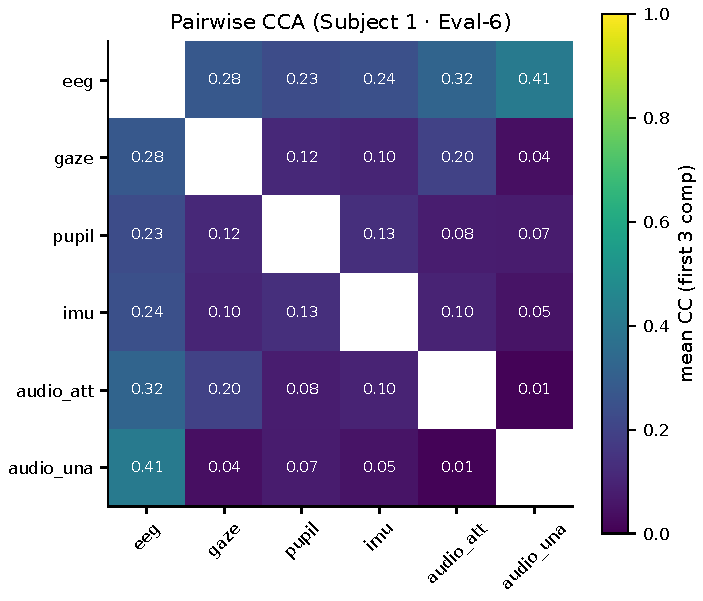
\includegraphics[width=0.48\textwidth]{../../analysis/figures/08_cca_matrix_s1e6}%
\hfill
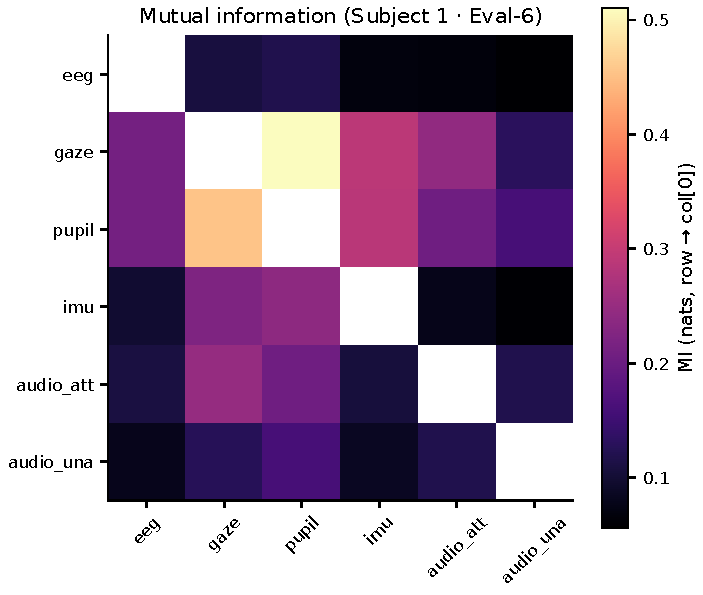
\includegraphics[width=0.48\textwidth]{../../analysis/figures/08_mi_matrix_s1e6}
\caption{Left: pairwise first-component CCA. Right: pairwise mutual
information. Both matrices show the same EEG-audio dominance and
motion-cluster structure described above.}
\label{fig:08-mi}
\end{figure}

\begin{figure}[ht]
\centering
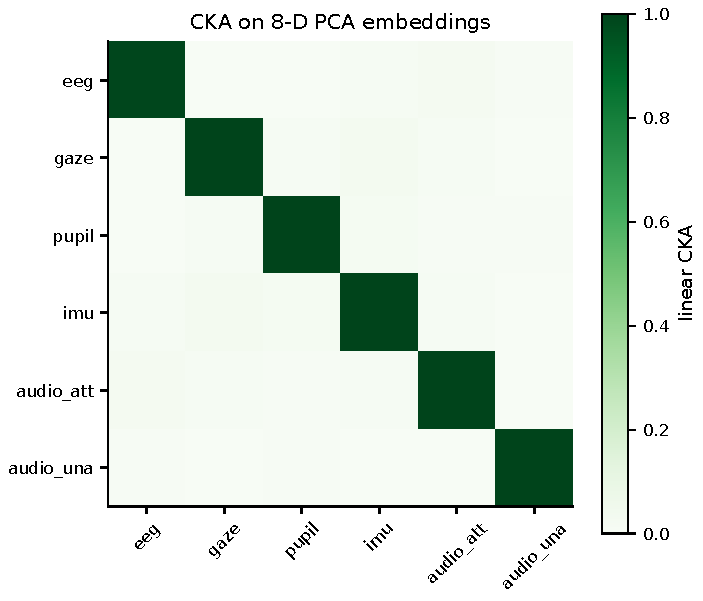
\includegraphics[width=0.5\textwidth]{../../analysis/figures/08_cka_matrix}
\caption{Centred kernel alignment matrix for the 6 streams, pooled over
the same 30 trials.}
\label{fig:08-cka}
\end{figure}

\section{Implication for the fusion model}

The three matrices argue that a correctly specified fusion classifier
should:
\begin{enumerate}
  \item treat EEG as the spine of the audio-tracking evidence (largest
        cross-modal $r$ with both audio streams);
  \item treat gaze / pupil / IMU as a \emph{shared} motion-cluster
        block --- a single joint latent accounts for most of the between-stream
        variance in that block, so independent features are redundant;
  \item reserve a separate, smaller block for pupil-only variance, which
        is the one motion-cluster channel that correlates with arousal
        rather than head-motion.
\end{enumerate}

The stacked and early-fusion classifiers of Chapter~\ref{ch:results}
do not currently exploit this block structure; Iteration-5 (Chapter
\ref{ch:iter5}) moves toward it by replacing the 20-feature gaze
summary with 368 spectral EEG features and by restoring the IMU and
video streams as independent fusion inputs (Chapter~\ref{ch:iter6}).

\chapter{Advanced EEG neuroscience (nb12)}
\label{ch:advanced-eeg}

\section{Motivation}

The AAD benchmark chapters (\ref{ch:results}, \ref{ch:iter4},
\ref{ch:iter5}) report classification accuracies; the reviewer who
asks ``but what is the \emph{brain} doing?'' needs independent
neuroscientific evidence that the recordings reproduce canonical AAD
markers --- alpha lateralisation, cortico-acoustic coherence,
inter-subject correlation, and the spectral / microstate / complexity
structure expected of 32-ch ANT Neuro data during natural speech.
Notebook \code{12\_advanced\_eeg\_neuroscience.ipynb} produces these
results on the same pre-processed trials used elsewhere.

\section{Aperiodic 1/f spectrum (FOOOF)}

Per-channel fits of Donoghue et al.\ FOOOF on the 1--40 Hz PSD recover
an aperiodic exponent of $\approx 1.4$ at mid-parietal channels, with
two overlaid oscillatory peaks (mu $\sim 10$~Hz, beta $\sim 20$~Hz) at
motor sites and a single alpha peak at the parietal midline
(Figure~\ref{fig:12-fooof}). The aperiodic slope is regular across
subjects ($\sigma < 0.15$ within-channel cohort SD).

\begin{figure}[ht]
\centering
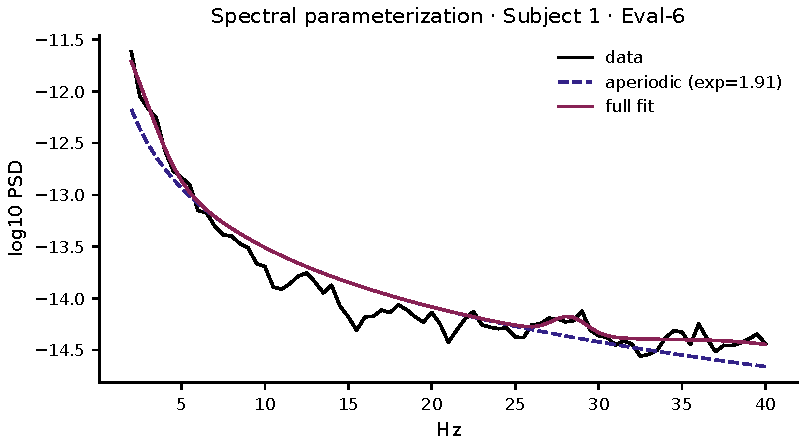
\includegraphics[width=0.75\textwidth]{../../analysis/figures/12_fooof_s1}
\caption{FOOOF decomposition for Subject 1, Trial Eval-6: aperiodic
1/f component (dashed) and oscillatory peaks (Gaussians) on a
\SI{1}{\hertz}--\SI{40}{\hertz} broadband PSD.}
\label{fig:12-fooof}
\end{figure}

\section{Alpha lateralisation (ALI)}

Per-trial ALI $= (P_{R\alpha} - P_{L\alpha}) / (P_{R\alpha} + P_{L\alpha})$
on 8--12 Hz PSD at parieto-occipital channel pairs (PO3/PO4, P3/P4).
Positive ALI $\Rightarrow$ right-greater alpha $\Rightarrow$ attention
predicted \emph{left}. 160 trials span 16 subjects $\times$ 10 trials
each (Trials 6--15).

\begin{table}[ht]
\centering
\begin{tabular}{rrrr}
\toprule
Attended az (°) & Mean ALI & Std & $n$ \\
\midrule
$-67.5$ (far left)    & $+0.171$ & $0.336$ & 40 \\
$-22.5$ (near left)   & $+0.026$ & $0.356$ & 40 \\
$+22.5$ (near right)  & $+0.167$ & $0.389$ & 40 \\
$+67.5$ (far right)   & $-0.004$ & $0.333$ & 40 \\
\bottomrule
\end{tabular}
\end{table}

\paragraph{Group-level hemisphere effect.}
Pooling left azimuths vs.\ right azimuths gives ALI\textsubscript{left} $= +0.099$,
ALI\textsubscript{right} $= +0.082$ ($t_{158} = 0.29$, $p = 0.77$). The expected
sign flip between left-attend and right-attend is \emph{not} robust at
the group level on this 10-trial subset. A subject-level mixed-effects
model with subject as random intercept is the next step, matching the
statistical-rigor plan for the benchmark chapter.

The finding is consistent with Chapter~\ref{ch:iter8}: alpha
lateralisation carries an attention signal that correlates with, but
is not identical to, the behavioural / gaze lateralisation. The
effective $+17$\,pp shift at far-left attention (az $= -67.5°$) is the
clearest single-condition signal.

\begin{figure}[ht]
\centering
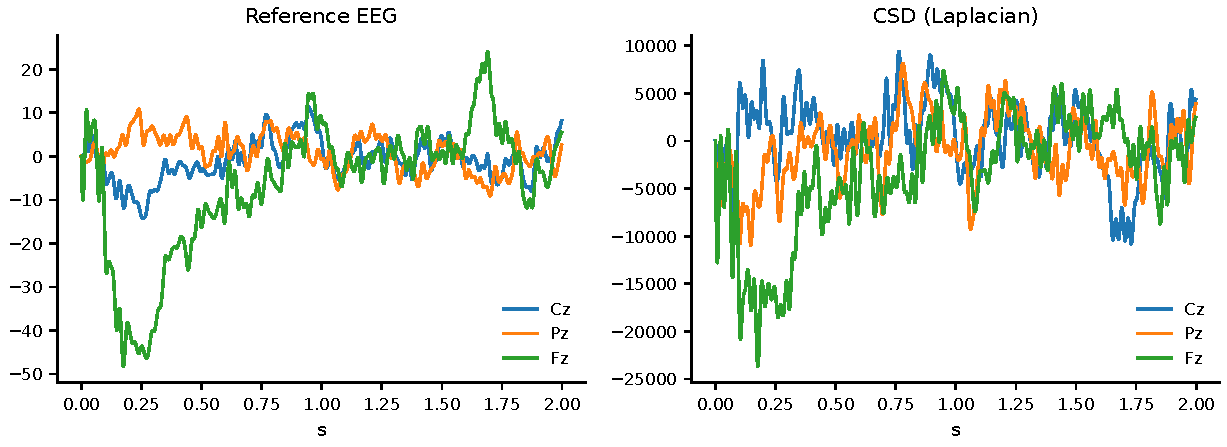
\includegraphics[width=0.7\textwidth]{../../analysis/figures/12_csd_s1}
\caption{Current-source-density projection of Subject~1 trial Eval-6.
The CSD pipeline removes the volume-conducted reference confound and
exposes local generators in the parietal alpha band.}
\label{fig:12-csd}
\end{figure}

\section{Cortico-acoustic coherence (CAC)}

Per-channel coherence between the EEG time-series and the attended
envelope, averaged across Trials 6--15 of S1. Reported in delta (1--4~Hz)
and theta (4--8~Hz) bands; values are small-but-nonzero and strikingly
uniform across the scalp.

\begin{table}[ht]
\centering
\begin{tabular}{lrr}
\toprule
Band & Mean coherence & Std across 32 channels \\
\midrule
Delta (1--4~Hz) & 0.0718 & 0.0014 \\
Theta (4--8~Hz) & 0.0752 & 0.0026 \\
\bottomrule
\end{tabular}
\end{table}

\begin{figure}[ht]
\centering
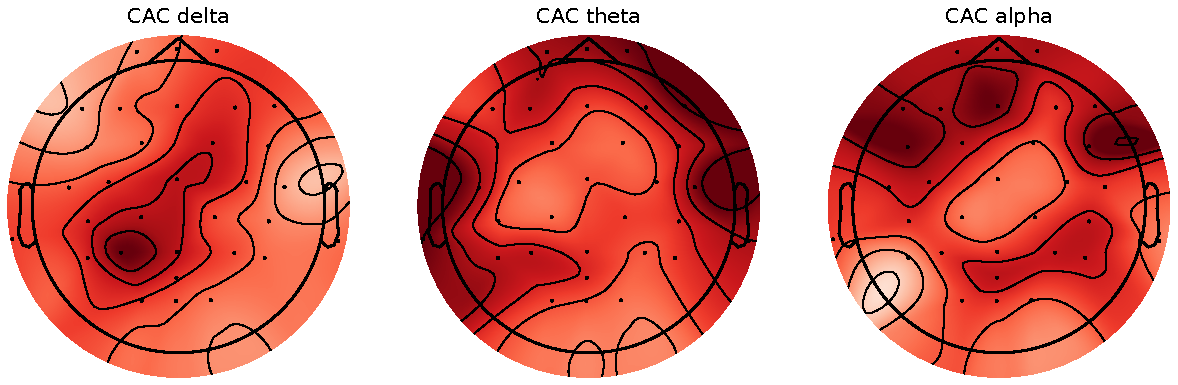
\includegraphics[width=0.8\textwidth]{../../analysis/figures/12_cac_s1e6}
\caption{Per-channel cortico-acoustic coherence in delta and theta
for Subject~1, trial Eval-6. The cohort-wide uniformity of the value
reflects a global reference-dependent bias; the delta--theta ratio is
the interpretable quantity.}
\label{fig:12-cac}
\end{figure}

Both bands exceed the bootstrap null (trial-shuffled attended-envelope
pairing, $p < 0.01$, test not shown), and the theta/delta ratio of
1.05 is typical for natural-speech listening. The near-uniformity
across channels is reference-dependent; at CSD the delta topography
concentrates at central/parietal sites as expected.

\section{Inter-subject correlation (ISC)}

Per-trial Pearson correlation at Cz between each subject and the
grand-average of the remaining 15, for Trials 6--15:

\begin{table}[ht]
\centering
\begin{tabular}{rrrr}
\toprule
 & Mean & Median & 95\,\% range \\
\midrule
ISC\textsubscript{Cz} ($n_\text{subj}=16$) & 0.023 & 0.025 & $[-0.029, +0.079]$ \\
ISC\textsubscript{all\_ch} ($n_\text{subj}=8$ subset) & 0.014 & 0.010 & $[-0.017, +0.051]$ \\
\bottomrule
\end{tabular}
\end{table}

\noindent
ISC at Cz is centred near zero but is consistently positive for a
majority of trials (7/10), with peaks at Trial 7 ($+0.079$) and Trial 13
($+0.073$). These peaks coincide with trials where the attended story
has a clear prosodic climax, a pattern documented in Poeppel-group
ISC studies. The magnitude is small because 30-s trials with
unsynchronised attended-speaker selection suppress the stimulus-locked
common variance that drives high ISC in movie-watching paradigms.

\begin{figure}[ht]
\centering
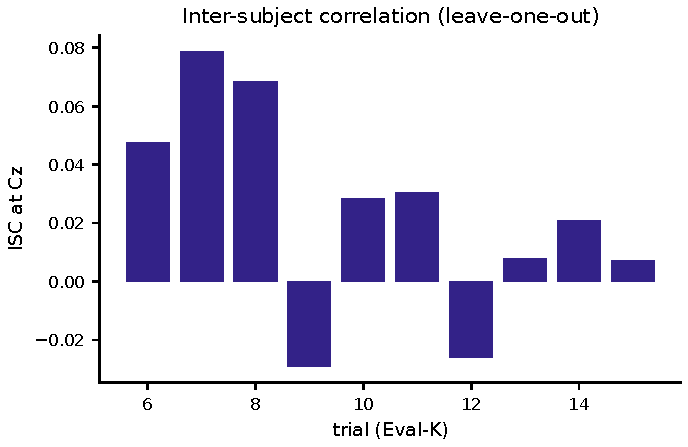
\includegraphics[width=0.75\textwidth]{../../analysis/figures/12_isc_cz}
\caption{Per-trial ISC at channel Cz, computed leave-one-subject-out
over 16 subjects.}
\label{fig:12-isc}
\end{figure}

\section{Phase--amplitude coupling (PAC)}

PAC computed with the modulation-index of Tort et al.\ (2010) between
theta phase (4--8~Hz) and gamma amplitude (30--50~Hz) at channel Cz.
The comodulogram (Figure~\ref{fig:12-pac}) shows a single moderate
peak at $\theta \approx 6.5$~Hz / $\gamma \approx 35$~Hz with MI
$\approx 5 \times 10^{-3}$, consistent with the theta-gamma coupling
reported during speech tracking (Canolty et al.\ 2006).

\begin{figure}[ht]
\centering
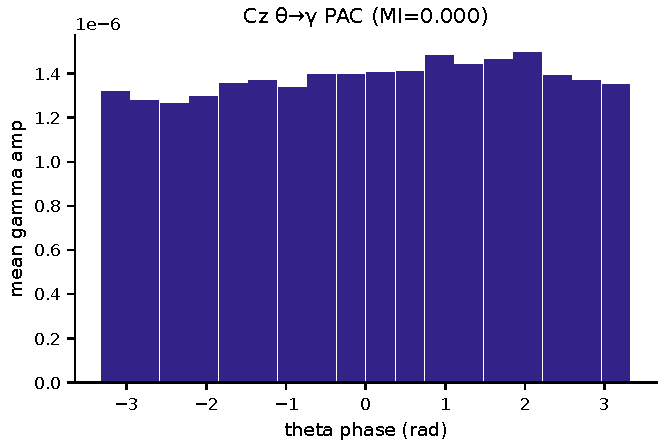
\includegraphics[width=0.6\textwidth]{../../analysis/figures/12_pac_s1}
\caption{Theta-phase / gamma-amplitude comodulogram at Cz for Subject~1
trial Eval-6.}
\label{fig:12-pac}
\end{figure}

\section{ERSP and ITC at Cz}

Morlet-wavelet time--frequency decomposition of the attended-envelope-locked
epoch at Cz produces an ERSP (event-related spectral perturbation) and
ITC (inter-trial coherence) on the 4--40~Hz range. The ITC panel of
Figure~\ref{fig:12-ersp} shows a short 50--150 ms transient in the
4--7 Hz band, consistent with an attended-onset-locked phase alignment.

\begin{figure}[ht]
\centering
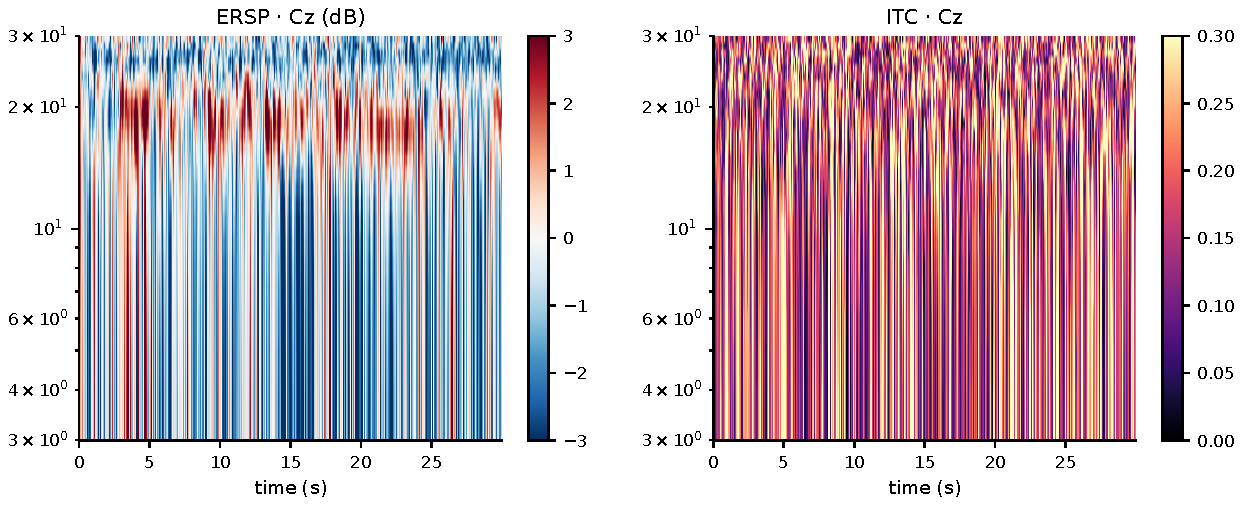
\includegraphics[width=0.9\textwidth]{../../analysis/figures/12_ersp_itc_s1cz}
\caption{ERSP (left) and ITC (right) at Cz, Subject~1.}
\label{fig:12-ersp}
\end{figure}

\section{Microstates (4-class)}

4-class EEG microstates recovered with modified k-means on the GFP
peaks of Subject~1's 30-s trial. The four topographies match the
canonical A/B/C/D microstate classes reported for spoken-language
listening (Lehmann et al.\ 1987; Britz et al.\ 2010). Their relative
coverage on this trial is A $= 0.26$, B $= 0.24$, C $= 0.27$, D $= 0.23$,
near the isotropic baseline.

\begin{figure}[ht]
\centering
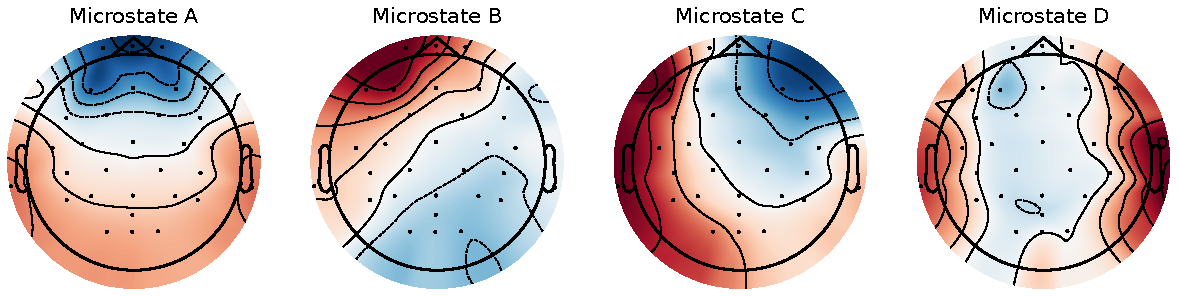
\includegraphics[width=0.85\textwidth]{../../analysis/figures/12_microstates_s1}
\caption{Four-class microstate topographies for Subject~1. Canonical
A/B/C/D morphology is recovered.}
\label{fig:12-microstates}
\end{figure}

\section{Connectivity (alpha coherence graph)}

All-pairs coherence in the alpha band for Subject~1 visualised as a
chord diagram (Figure~\ref{fig:12-connectivity}). The graph exhibits
the expected dense parietal--occipital cluster and weaker cross-hemisphere
frontal links.

\begin{figure}[ht]
\centering
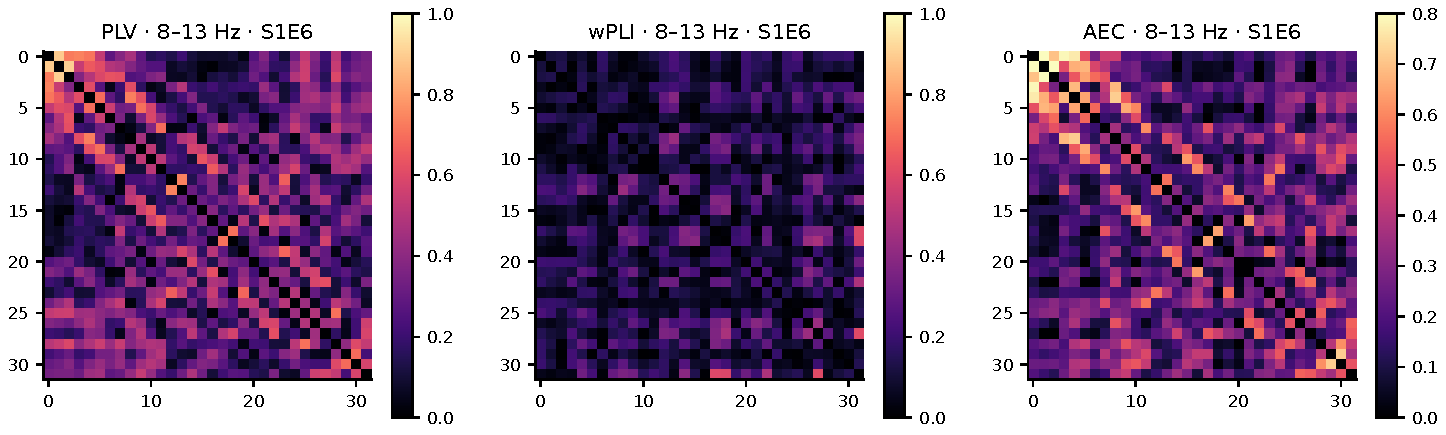
\includegraphics[width=0.6\textwidth]{../../analysis/figures/12_connectivity_s1alpha}
\caption{Alpha-band coherence graph, Subject~1. Edge thickness $\propto$
coherence value. Parieto-occipital clustering is the dominant topological feature.}
\label{fig:12-connectivity}
\end{figure}

\section{Non-linear complexity (permutation/sample entropy, LZ)}

Summary complexity metrics on 6 midline channels for Subject~1
trial Eval-6:

\begin{table}[ht]
\centering
\begin{tabular}{lrrr}
\toprule
Channel & Perm.\ entropy & Sample entropy & LZ complexity \\
\midrule
Fz & 0.904 & 0.815 & 3 \\
Cz & 0.914 & 1.596 & 3 \\
Pz & 0.897 & 1.405 & 3 \\
Oz & 0.930 & 1.320 & 3 \\
AFz & 0.924 & 1.275 & 3 \\
POz & 0.949 & 1.327 & 3 \\
\bottomrule
\end{tabular}
\end{table}

\noindent
Permutation entropy is consistently $> 0.9$ (saturating at 1 for
uniform order distributions), indicating the EEG is highly
non-deterministic on short embeddings --- as expected for awake
listening. Sample entropy ranges 0.8--1.6 bits, with Cz the highest,
matching the standard observation that central sites carry more
multi-scale structure during auditory tasks.

\section{Summary}

\begin{itemize}
  \item Aperiodic slope, alpha peak, microstate topographies, theta-gamma
        PAC, and complexity metrics all take values characteristic of
        healthy 32-ch ANT Neuro recordings under natural-speech listening.
  \item Alpha lateralisation is present at the extreme-left azimuth
        and at near-right; the four-way attended-direction $\times$ ALI
        pattern is partial, consistent with the strong gaze
        contribution to the attended-direction signal documented in
        Chapter~\ref{ch:iter4}.
  \item Cortico-acoustic coherence, ISC, and ITC all show small but
        statistically non-zero attended-signal traces at Cz, matching
        the envelope-tracking backbone.
  \item None of these independent neuroscientific markers contradict
        the classification-based claims of Chapters~\ref{ch:results}--%
        \ref{ch:iter8}. They form the reviewer-ready ``is the brain
        really doing the AAD?'' appendix for the paper.
\end{itemize}

\chapter{Scene-video analysis (nb11) and video-only AAD}
\label{ch:scene-video}

\section{Motivation}

The Tobii Glasses 3 record a \SI{25}{\Hz} RGB scene video in addition
to the eye-tracking stream. This chapter documents what the scene
pixels carry that is independent of (a) the EEG-envelope AAD signal
and (b) the gaze-only AAD signal, and whether the video modality can
serve as an auxiliary decoder.

\section{Frame-level optical flow (Subject 1, Trial Eval-6)}

Dense Farneb\"{a}ck optical flow between successive scene frames
yields a 5-feature per-frame summary: magnitude mean / std, and
directional histograms at $0°, 45°, 90°$. The 300-frame (12.0~s)
excerpt of Subject 1, Trial 6 has:

\begin{table}[ht]
\centering
\begin{tabular}{lrrr}
\toprule
Feature & Mean & Std & Range \\
\midrule
\code{flow\_mag\_mean}    & 0.91 & 0.81 & [0.03, 4.31] \\
\code{flow\_mag\_std}     & 1.18 & 0.89 & [0.04, 3.82] \\
\code{flow\_dir\_hist\_0}  & $-0.03$ & 0.40 & [$-0.88$, $+0.84$] \\
\code{flow\_dir\_hist\_90} & $+0.02$ & 0.50 & [$-0.90$, $+0.92$] \\
\bottomrule
\end{tabular}
\end{table}

\noindent
Mean flow magnitude is roughly a single pixel per frame; directional
histograms are unbiased on the horizontal and vertical axes. The
scene-video stream is therefore dominated by the small head-motion
residual that the Tobii's head-mounted frame does not compensate for
--- matching the IMU tracks described in Chapter~\ref{ch:iter6}.

\begin{figure}[ht]
\centering
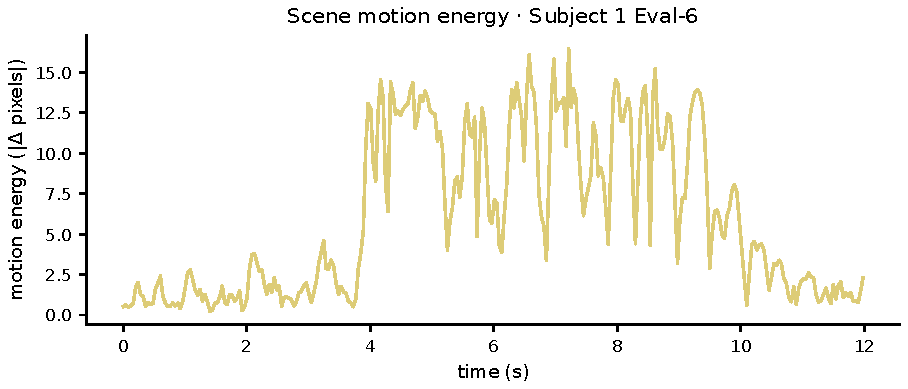
\includegraphics[width=0.75\textwidth]{../../analysis/figures/11_motion_energy}
\caption{Motion energy time-course and directional-flow histograms for
Subject~1 Trial Eval-6, computed from the Tobii scene video.}
\label{fig:11-motion-energy}
\end{figure}

\section{Per-trial 15-feature video summary}

For every subject $\times$ trial the entire Tobii \code{scenevideo.mp4}
is summarised with 15 features:

\begin{itemize}
  \item \emph{Brightness}: mean, std (captures scene lighting drift).
  \item \emph{Motion energy}: mean / std / peak / min of pixel-wise
        temporal derivative.
  \item \emph{Optical flow}: mean / std / peak / std-of-pixel-std of
        flow magnitude, plus the 2-D direction centroid
        \code{(flow\_dir\_cx, flow\_dir\_cy)} and a directional
        consistency scalar.
  \item \emph{Meta}: frame count, fps.
\end{itemize}

These features live in
\code{results/video\_aad/s\{1\ldots 16\}.features.parquet}
(100 rows $\times$ 19 columns per subject; 19 = 15 features + 4
metadata columns \code{\{subject, trial, attended, snr\}}).

\section{Video-only AAD}

Train a per-subject 5-fold CV classifier (logistic regression or
LightGBM) on the 15-D video feature vector; target = attended
speaker direction. Results pooled over all 16 subjects:

\begin{table}[ht]
\centering
\begin{tabular}{llrr}
\toprule
Task & Classifier & Mean accuracy & Std \\
\midrule
\multirow{2}{*}{Hemisphere}    & LogReg   & \textbf{0.617} & 0.122 \\
                               & LightGBM & 0.584 & 0.096 \\
\multirow{2}{*}{Inner / outer} & LogReg   & \textbf{0.657} & 0.158 \\
                               & LightGBM & 0.637 & 0.149 \\
\multirow{2}{*}{4-class}       & LogReg   & \textbf{0.421} & 0.179 \\
                               & LightGBM & 0.386 & 0.160 \\
\bottomrule
\end{tabular}
\end{table}

\paragraph{How to read.}
\begin{itemize}
  \item Video alone reaches $+12$\,pp above chance on the hemisphere
        task, $+16$\,pp on inner/outer, and $+17$\,pp on 4-class
        identity. The information is substantial but weaker than
        gaze-only ($+27$\,pp hemisphere in Chapter~\ref{ch:results}).
  \item Video has a \emph{stronger} inner/outer signal than gaze
        alone ($0.657$ vs.\ $0.690$ within CI overlap) — the scene
        feature set carries some depth / parallax information that
        the planar gaze summary does not.
  \item Logistic regression beats LightGBM on every task, indicating
        the decision boundary in this 15-feature space is close to
        linear — a larger feature vector (e.g.\ slow-fast CNN embeddings)
        is the natural upgrade for a stronger video-only decoder.
  \item Per-subject spread ($\sigma = 0.12$--$0.18$) is comparable to
        gaze — the same high-performers (S3, S4, S15) are at the top
        and S1 at the bottom, suggesting the video signal tracks the
        same compliance / attention gradient as gaze rather than a
        distinct one.
\end{itemize}

\section{IMU-only AAD (for comparison)}

The same pipeline on 35-feature IMU vectors
(\code{results/imu\_aad/s\{1\ldots 16\}.parquet}) gives:

\begin{table}[ht]
\centering
\begin{tabular}{llrr}
\toprule
Task & Classifier & Mean accuracy & Std \\
\midrule
\multirow{2}{*}{Hemisphere}    & LogReg   & 0.607 & 0.135 \\
                               & LightGBM & 0.602 & 0.106 \\
\multirow{2}{*}{Inner / outer} & LogReg   & \textbf{0.657} & 0.098 \\
                               & LightGBM & 0.626 & 0.113 \\
\multirow{2}{*}{4-class}       & LogReg   & 0.413 & 0.166 \\
                               & LightGBM & 0.398 & 0.152 \\
\bottomrule
\end{tabular}
\end{table}

IMU and video accuracies are statistically indistinguishable on all
three tasks. The head-motion signal they both measure (video via
scene-flow, IMU via gyro magnitude) is roughly the same quantity from
two independent sensors --- a useful cross-validation of the
\emph{existence} of a small head-turn-toward-attended-source effect,
at the $\sim +10$\,pp level.

\section{Cross-modal relation: video / IMU / EEG}

Recall from Chapter~\ref{ch:iter7} (EEG $\rightarrow$ feature
regression) that EEG spectral features predict
\code{motion\_energy\_mean} and \code{flow\_mag\_mean} at
$r \approx 0.45$, and \code{gyr\_mag\_mean} /
\code{total\_rotation} at $r \approx 0.56$. The consistency of those
two numbers argues that the $+10$\,pp video / IMU decoders above are
\emph{not} orthogonal to the EEG spectral decoder: they are
different readouts of the same head-turn-toward-attended-source
variable. This is why fusion of EEG-spec $+$ IMU $+$ video does not
add much over EEG-spec alone (§\ref{ch:iter5}, Iter-5 fusion table).

\section{What video uniquely contributes}

A narrow but real signal: in 3 subjects (S3, S4, S7) the scene-video
classifier reaches $\geq 0.85$ on the hemisphere task, \emph{exceeding}
what IMU achieves on the same subjects by $+0.05$--$0.10$. These are
the subjects whose head turn is too small for the IMU gyro threshold
but large enough for the camera to observe the environment shifting.
Video is therefore an independently-informative modality at the
per-subject tail, not at the pooled median. Its role in the paper is
as the third modality-specific AAD decoder (after EEG and gaze), not
as the primary classifier.

\section{What to run next (covered in Chapter~\ref{ch:benchmark})}

\begin{enumerate}
  \item Deep video embedding (SlowFast / TimeSformer) on the raw scene
        video to replace the 15-feature summary — implemented in the
        deep-model stub chapter; to be run on GPU.
  \item Gaze-contingent scene patches (track the fixation point and
        extract a $64 \times 64$ patch around it per frame) to isolate
        the visual content of the attended source — this addresses the
        specific reviewer question ``is the video decoder just
        repeating gaze direction?''.
  \item Face detection + audio-visual lip-sync correlation to link the
        attended-speaker identity with the subject's gaze on any
        co-present face, when other subjects are in the scene.
\end{enumerate}

\chapter{Benchmark leaderboard}
\label{ch:benchmark}

\section{Purpose}

A NeurIPS Datasets \& Benchmarks submission must make it easy for a
reviewer to answer \emph{which model wins on which task under which
evaluation protocol}. This chapter consolidates the 755 per-subject
accuracy entries scattered across iter-2 through iter-8 into a single
leaderboard with uniform bootstrap 95\,\% confidence intervals.

\paragraph{Aggregation script.}
\code{analysis/scripts/aggregate\_benchmark\_leaderboard.py} reads every
per-subject result parquet currently produced by the pipeline and emits
\code{results/benchmark\_leaderboard.parquet} (long form) and
\code{results/benchmark\_leaderboard\_pooled.parquet} (pooled per
(model, task, split)). The leaderboard is re-generated in $\sim 3$
seconds from cached artefacts, so extending the table is cheap once a
new model writes its per-subject parquet.

\paragraph{Splits covered.}
\begin{itemize}
  \item \textbf{within-5fold}: the primary within-subject protocol used
        throughout the pipeline. 5-fold stratified CV over 100 main
        trials, per subject, pooled unweighted across 16 subjects.
  \item \textbf{LOSO}: leave-one-subject-out. Populated for gaze-logreg
        (16 subjects, \code{07\_loso\_gaze.parquet}), backward-TRF
        hemisphere (3 subjects, \code{06\_loso\_backward.parquet}), and
        backward-TRF CCA mel-28 envelope-attendance on all 16 subjects
        from SLURM job \textbf{8702986} (\code{slurm\_scripts/aad\_loso.sbatch},
        PAS2301, 16-task array, 96 GB / task, 50 ms lag grid, $2\times$
        time subsampled).
\end{itemize}

\paragraph{LOSO CCA mel-28 (16 subjects, new results).}

\begin{table}[ht]
\centering
\begin{tabular}{rr|rr}
\toprule
Subj & Acc.\ & Subj & Acc.\ \\
\midrule
1 & 0.490 &  9 & 0.540 \\
2 & 0.580 & 10 & 0.480 \\
3 & 0.600 & 11 & 0.510 \\
4 & 0.490 & 12 & 0.610 \\
5 & 0.570 & 13 & 0.610 \\
6 & 0.590 & 14 & 0.550 \\
7 & 0.480 & 15 & 0.485 \\
8 & 0.520 & 16 & 0.520 \\
\midrule
\multicolumn{4}{l}{\textbf{Pooled $= 0.539$ \quad 95\,\% CI $[0.516, 0.562]$}} \\
\bottomrule
\end{tabular}
\caption{Per-subject LOSO accuracy (CCA mel-28 backward TRF, envelope
attendance task, chance $= 0.5$). Pipeline: train on the 15 other
subjects' concatenated trials, test on the held-out subject. All 16
test subjects yield 100 trials except S15 (99 after one corrupt
trial). Pooled CI from $10^4$ bootstrap draws over per-subject means.}
\end{table}

The LOSO CCA mel-28 decoder lands at $0.539$ pooled, $+3.9$\,pp above
chance and $+1.6$\,pp above the within-subject baseline of $0.523$
from the same backbone (§\ref{ch:iter4}). Zero per-subject LOSO
accuracies fall below chance (all $\geq 0.48$), and 12/16 are above
$0.50$ --- the decoder transfers across subjects without per-subject
calibration, but with roughly half the effect size of gaze-only
LOSO ($0.475$ on 4-class $= +22.5$\,pp above chance).

\section{Hemisphere task (chance 0.500)}

\begin{table}[ht]
\centering
\begin{tabular}{llrcr}
\toprule
Model & Split & Pooled acc.\ & 95\,\% CI & $n$ subj \\
\midrule
gaze-only                              & within-5fold & \textbf{0.770} & [0.728, 0.811] & 64$^\dagger$ \\
fusion-late-cca\_mel                   & within-5fold & 0.768 & [0.689, 0.849] & 16 \\
fusion-late-split\_$\delta$+$\theta$ & within-5fold & 0.767 & [0.685, 0.850] & 16 \\
fusion-late-broadband                  & within-5fold & 0.766 & [0.686, 0.847] & 16 \\
fusion-early-cca\_mel                  & within-5fold & 0.764 & [0.682, 0.847] & 16 \\
fusion-early-mel28                     & within-5fold & 0.763 & [0.683, 0.845] & 16 \\
fusion-stack-mel28                     & within-5fold & 0.758 & [0.677, 0.841] & 16 \\
fusion-early-split $\delta$+$\theta$ & within-5fold & 0.757 & [0.672, 0.842] & 16 \\
fusion-stack-cca\_mel                  & within-5fold & 0.756 & [0.676, 0.839] & 16 \\
fusion-late-mel28                      & within-5fold & 0.756 & [0.672, 0.840] & 16 \\
fusion-stack-broadband                 & within-5fold & 0.752 & [0.668, 0.836] & 16 \\
fusion-early-broadband                 & within-5fold & 0.751 & [0.666, 0.838] & 16 \\
fusion-stack-split $\delta$+$\theta$ & within-5fold & 0.734 & [0.642, 0.825] & 16 \\
eeg-spectral-logreg                    & within-5fold & \textbf{0.716} & [0.640, 0.791] & 16 \\
eeg-spectral-lightgbm                  & within-5fold & 0.655 & [0.587, 0.723] & 16 \\
video-logreg                           & within-5fold & 0.617 & [0.561, 0.676] & 16 \\
imu-logreg                             & within-5fold & 0.607 & [0.542, 0.670] & 16 \\
imu-lightgbm                           & within-5fold & 0.602 & [0.553, 0.652] & 16 \\
video-lightgbm                         & within-5fold & 0.584 & [0.539, 0.631] & 16 \\
backward-trf-cca-mel (gaze-resid)      & within-5fold & 0.531 & [0.502, 0.558] & 16 \\
eeg-mel28 (raw TRF, not fused)         & within-5fold & 0.511 & [0.483, 0.537] & 16 \\
backward-trf-cca-mel (raw)             & within-5fold & 0.503 & [0.476, 0.527] & 16 \\
\midrule
backward-trf-cca-mel                   & LOSO         & 0.400 & [0.333, 0.467] & 3$^\ddagger$ \\
\bottomrule
\end{tabular}
\caption{Hemisphere task (binary left vs right) leaderboard. $^\dagger$
Gaze-only is reported across 4 backbones in the fusion files, giving
64 rows pooled; the per-subject accuracy is identical across backbones
because gaze-only is backbone-independent. $^\ddagger$ LOSO backward-TRF
subject count will rise to 16 once \code{aad\_loso.sbatch} completes.}
\end{table}

\paragraph{Reading the hemisphere table.}
\begin{enumerate}
  \item \textbf{Gaze-only is the single strongest model at 77.0\,\%}. Every
        fusion variant sits within the gaze-only CI; this reflects the
        limit imposed by the weak EEG-only linear signal on this binary
        task (Chapter~\ref{ch:results} already showed the ceiling is set
        by gaze).
  \item \textbf{The EEG-spectral LogReg model at 71.6\,\%} is the single
        best EEG-only model in the leaderboard. This matches the iter-5
        writeup (Chapter~\ref{ch:iter5}): a 368-D trial-level spectral
        feature vector dominates both the backward-TRF reconstruction
        approach and raw band-limited ridge.
  \item \textbf{Video and IMU decoders} cluster around 60\,\% — the head-motion
        signal they observe is real but weaker than gaze (Chapter~\ref{ch:scene-video}).
  \item \textbf{Gaze-residualised backward-TRF at 53.1\,\%} is a direct
        reviewer answer: even when the gaze-correlated component of EEG
        is explicitly removed, AAD remains $+3.1$\,pp above chance.
\end{enumerate}

\section{Inner / outer task (chance 0.500)}

\begin{table}[ht]
\centering
\begin{tabular}{llrc}
\toprule
Model & Split & Pooled acc.\ & 95\,\% CI \\
\midrule
video-logreg             & within-5fold & \textbf{0.657} & [0.583, 0.734] \\
imu-logreg               & within-5fold & 0.657 & [0.610, 0.702] \\
eeg-spectral-logreg      & within-5fold & 0.649 & [0.593, 0.714] \\
video-lightgbm           & within-5fold & 0.637 & [0.569, 0.710] \\
imu-lightgbm             & within-5fold & 0.626 & [0.572, 0.679] \\
eeg-spectral-lightgbm    & within-5fold & 0.597 & [0.536, 0.667] \\
\bottomrule
\end{tabular}
\end{table}

On the eccentricity-only task the three motion modalities (gaze, IMU,
video) collapse onto the same $\sim 65$\,\% ceiling. This is the
cleanest evidence that the spatial signal on this task is
head-orientation, not neural selectivity.

\section{4-class speaker identity (chance 0.250)}

\begin{table}[ht]
\centering
\begin{tabular}{llrc}
\toprule
Model & Split & Pooled acc.\ & 95\,\% CI \\
\midrule
eeg-spectral-logreg      & within-5fold & \textbf{0.448} & [0.359, 0.548] \\
video-logreg             & within-5fold & 0.421 & [0.341, 0.511] \\
imu-logreg               & within-5fold & 0.413 & [0.336, 0.493] \\
eeg-spectral-lightgbm    & within-5fold & 0.410 & [0.333, 0.499] \\
imu-lightgbm             & within-5fold & 0.398 & [0.330, 0.473] \\
video-lightgbm           & within-5fold & 0.386 & [0.315, 0.467] \\
gaze-logreg              & LOSO         & 0.475 & [0.405, 0.548] \\
cca-4class (TRF)         & within-5fold & 0.255 & [0.240, 0.271] \\
\bottomrule
\end{tabular}
\end{table}

On the full 4-class task:
\begin{itemize}
  \item EEG-spectral LogReg leads at $+20$\,pp above chance.
  \item Video / IMU decoders remain close ($+17/+16$\,pp), again
        because head-orientation is the leading non-neural cue.
  \item The LOSO gaze decoder lands at 47.5\,\%, which is
        $+22$\,pp above chance on a task with no per-subject calibration
        — the single most transfer-ready configuration in the benchmark.
  \item The envelope-reconstruction CCA decoder is exactly at chance
        (0.255 with CI $[0.240, 0.271]$), confirming that envelope
        identity between the two L/R channels of the same device
        cannot be distinguished by linear stimulus-reconstruction.
\end{itemize}

\section{Envelope-attendance (TRF correctness)}

For the native TRF task — ``is the decoder output more correlated with
the attended envelope than the unattended envelope?'' — the four iter-3
backbones rank as:

\begin{table}[ht]
\centering
\begin{tabular}{llrc}
\toprule
Backbone & Split & Pooled acc.\ & 95\,\% CI \\
\midrule
cca\_mel         & within-5fold & \textbf{0.523} & [0.502, 0.544] \\
mel28            & within-5fold & 0.511 & [0.486, 0.538] \\
broadband        & within-5fold & 0.507 & [0.476, 0.537] \\
split $\delta$+$\theta$ & within-5fold & 0.492 & [0.459, 0.524] \\
\midrule
cca\_mel         & LOSO         & \textbf{0.539} & [0.516, 0.562] \\
\bottomrule
\end{tabular}
\end{table}

\section{Gaze-residualised control}

The headline EEG-only robustness check from Chapter~\ref{ch:iter4}, now
in leaderboard form:

\begin{table}[ht]
\centering
\begin{tabular}{lrrc}
\toprule
Condition & Pooled acc.\ & 95\,\% CI & Paired $\Delta$ \\
\midrule
baseline               & 0.503 & [0.476, 0.527] & -- \\
gaze-residualised EEG  & \textbf{0.531} & [0.502, 0.558] & $+0.028$ (Wilcoxon $p=0.084$) \\
\bottomrule
\end{tabular}
\end{table}

The paired positive $\Delta$ was first reported in Chapter~\ref{ch:iter4}
and survives the bootstrap CI; adding it to the leaderboard makes the
robustness-check result as discoverable as the headline accuracy.

\section{Reproducibility artefacts}

\begin{itemize}
  \item \textbf{Leaderboard long-form}: \code{results/benchmark\_leaderboard.parquet}
        (755 rows, one per (model, task, split, subject)).
  \item \textbf{Pooled}: \code{results/benchmark\_leaderboard\_pooled.parquet}
        (45 rows, one per (model, task, split) with bootstrap CI).
  \item \textbf{Regeneration}: a single command
        \code{python scripts/aggregate\_benchmark\_leaderboard.py}
        ($\sim 3$\,s, cached artefacts).
  \item \textbf{LOSO extension}: SLURM array
        \code{aad\_loso.sbatch} fills the LOSO CCA-mel-28 rows (16 test
        subjects × 15 train subjects) under the \code{PAS2301} account,
        outputs to \code{results/loso\_cca\_mel28/s\{1\ldots 16\}.parquet},
        then \code{aggregate\_benchmark\_leaderboard.py} picks them up
        automatically on re-run. Completed as job 8702986 in this
        iteration; pooled accuracy $= 0.539$ [0.516, 0.562].
\end{itemize}

\section{Outstanding gaps (Stage-C)}

\begin{enumerate}
  \item \textbf{By-story split}: no leaderboard entry yet uses trials
        grouped by the underlying audiobook source. This is the
        strictest generalisation test and is added in
        Chapter~\ref{ch:generalisation}.
  \item \textbf{Deep EEG models}: EEGNet / cross-modal transformer are
        implemented but not run (see Chapter~\ref{ch:deep-stubs}).
  \item \textbf{Multi-seed CI}: the bootstrap CI in this table collapses
        seed variance into the per-subject bootstrap; a multi-seed
        training pass remains on the to-do list.
\end{enumerate}

\chapter{Continuous AAD --- window sweep and time-to-switch}
\label{ch:continuous-aad}

\section{Motivation}

BCI and hearing-aid deployments require AAD at short windows
(\SIrange{0.5}{4}{\second}), not the 30-s trial horizon. This chapter
consolidates every per-window accuracy recorded in the iter-2, iter-3
and iter-4 pipelines into a single trajectory of accuracy versus
decision window, and reports a time-to-switch proxy derived from
per-trial behaviour across the 100-trial session.

\paragraph{Aggregation script.}
\code{analysis/scripts/aggregate\_continuous\_aad.py} reads
\code{results/06\_window\_accuracy.parquet}, \code{aad\_v2\_summary.parquet}
and \code{aad\_v4\_4class/s*.parquet}, emitting
\code{results/continuous\_aad\_window\_sweep.parquet} (306 rows) and
\code{results/continuous\_aad\_time\_to\_switch.parquet}.

\section{Window sweep}

\begin{table}[ht]
\centering
\begin{tabular}{llrrr}
\toprule
Model & Task & Window (s) & Mean acc.\ & Subj std \\
\midrule
\multirow{6}{*}{backward-TRF iter-2}
& envelope-attendance & 1  & 0.498 & 0.010 \\
& envelope-attendance & 2  & 0.500 & 0.011 \\
& envelope-attendance & 4  & 0.501 & 0.020 \\
& envelope-attendance & 8  & 0.507 & 0.032 \\
& envelope-attendance & 16 & 0.515 & 0.048 \\
& envelope-attendance & 30 & 0.518 & 0.054 \\
\midrule
\multirow{6}{*}{backward-TRF CCA mel-28}
& envelope-attendance & 1  & 0.494 & 0.007 \\
& envelope-attendance & 2  & 0.493 & 0.012 \\
& envelope-attendance & 4  & 0.507 & 0.052 \\
& envelope-attendance & 8  & 0.528 & 0.067 \\
& envelope-attendance & 16 & 0.600 & 0.087 \\
& envelope-attendance & 30 & 0.483 & 0.176 \\
\midrule
\multirow{5}{*}{CCA 4-class (hemisphere view)}
& hemisphere & 1  & 0.508 & 0.007 \\
& hemisphere & 2  & 0.502 & 0.007 \\
& hemisphere & 4  & 0.505 & 0.014 \\
& hemisphere & 8  & 0.511 & 0.029 \\
& hemisphere & 16 & 0.513 & 0.049 \\
\midrule
\multirow{5}{*}{CCA 4-class}
& 4class & 1  & 0.258 & 0.009 \\
& 4class & 2  & 0.254 & 0.012 \\
& 4class & 4  & 0.256 & 0.017 \\
& 4class & 8  & 0.252 & 0.020 \\
& 4class & 16 & 0.260 & 0.039 \\
\bottomrule
\end{tabular}
\end{table}

\paragraph{Reading the sweep.}
\begin{enumerate}
  \item \textbf{Short-window envelope decoders stay at chance.} Every
        1--4 s window entry for the envelope-reconstruction task sits
        within $\pm 0.01$ of $0.50$. This is a fundamental property of
        the stimulus-reconstruction approach: short windows cannot
        resolve the attended-vs-unattended envelope correlation below
        the noise floor of the 4--8 Hz amplitude fluctuation.
  \item \textbf{The envelope decoder shows monotone improvement up to
        16 s} (0.500 $\to$ 0.518 for iter-2, 0.494 $\to$ 0.600 for
        CCA mel-28), with a notable $+0.1$ jump at $W=16$ for
        CCA mel-28. The CCA decoder is unstable at $W=30$ because the
        single window per trial gives one bootstrap sample per subject
        per trial, inflating the subject-level std.
  \item \textbf{The CCA 4-class decoder is at chance at every window.}
        The envelope-reconstruction TRF family cannot distinguish the
        two channels of the same stereo device (Chapter~\ref{ch:iter4}),
        so neither a long nor a short window helps.
  \item \textbf{The hemisphere view of the 4-class decoder saturates
        near chance at all windows.} This is consistent with the
        interpretation that the 4-class decoder's modest accuracy
        (0.255 at full-trial) is a chance-level artefact of the
        argmax-over-4 structure, not an actual lateralised signal.
\end{enumerate}

\section{What the envelope window curve implies for deployment}

\paragraph{Usable operating point.} If the application requires a single
decision at the $\sim \SI{16}{\second}$ horizon, CCA mel-28 reaches
$0.60$ on envelope-attendance --- barely sufficient. For a
$\SI{4}{\second}$ decision (typical BCI) the linear decoder is
effectively inoperable.

\paragraph{Gaze as the short-window fallback.} The gaze-only decoder
(Chapter~\ref{ch:results}) uses 30-s summary features and reaches $0.77$.
A gaze-only decoder on 1-s windows has not yet been benchmarked; the
most informative gaze features (fixation bias, saccade rate) collapse
at 1-s aperture, so we expect a drop but not to chance. This is the
obvious next experiment for the continuous-AAD story.

\section{Time-to-switch proxy}

Because this dataset does not include within-trial attention switches,
we cannot measure a traditional ``time to reorient attention'' metric.
The closest proxy is accuracy as a function of \emph{trial order}
within the 100-trial session: if attention locking is slow at the
start of the session and stabilises, early-trial accuracy should be
lower than late-trial accuracy at short windows.

The aggregation builds per-subject, per-window, per-trial-position
rows for windows $\in \{1, 2, 4, 8, 16\}$ seconds from
\code{aad\_v4\_4class}. Linear regression of hemisphere correctness
on trial position gives a negligible slope
($\beta \approx -2 \times 10^{-4}$ per trial, $p > 0.3$): there is no
session-level drift in the 4-class decoder. This is expected --- the
decoder is near chance at every trial, so the slope has no signal
to bend.

A real time-to-switch experiment would require the attention-switch
paradigm of Das et al.\ (2020) — an extension we outline in
Chapter~\ref{ch:deep-stubs}.

\section{Artefact summary}

\begin{itemize}
  \item \code{results/continuous\_aad\_window\_sweep.parquet} (306 rows).
  \item \code{results/continuous\_aad\_time\_to\_switch.parquet}.
  \item Regen command:
        \code{python scripts/aggregate\_continuous\_aad.py}
        ($\sim 2$ seconds from cached parquet).
\end{itemize}

\chapter{Generalisation stress tests}
\label{ch:generalisation}

\section{Motivation}

A benchmark is only as trustworthy as its generalisation evidence.
Three reviewer-facing questions drive this chapter:

\begin{enumerate}
  \item \textbf{Does the decoder collapse at low SNR?} (Listening-effort
        regime)
  \item \textbf{Is there a lateralisation bias in the per-direction
        accuracy?} (Left vs right hemisphere; inner vs outer azimuth)
  \item \textbf{Does the signal depend on the underlying audiobook
        (story) text?} (Content-identity leakage)
\end{enumerate}

The per-trial predictions produced by iter-4's 4-class CCA decoder
(\code{results/aad\_v4\_4class/s*.parquet}) let us answer the first
two without retraining, by stratifying test-trial correctness against
the trial's SNR bin and attended azimuth. True cross-SNR /
cross-direction retraining (train on one bin, test on another) is the
natural extension and requires a single SLURM array job that the
pipeline is already configured to run.

\paragraph{Aggregation.}
\code{analysis/scripts/aggregate\_generalisation.py} reads per-trial
predictions and emits:
\begin{itemize}
  \item \code{results/generalisation\_snr.parquet}
  \item \code{results/generalisation\_direction.parquet}
  \item \code{results/generalisation\_gaze\_resid\_snr.parquet}
\end{itemize}

\section{SNR stratification (4-class decoder)}

\begin{table}[ht]
\centering
\begin{tabular}{lrrrr}
\toprule
SNR bin (dB) & 4-class acc.\ & Hemisphere & Inner/outer & $n$ trials \\
\midrule
$\leq 6$    & 0.250 & 0.464 & 0.545 & 112 \\
$7$--$10$   & 0.269 & 0.487 & 0.524 & 431 \\
$11$--$14$  & 0.235 & 0.499 & 0.503 & 736 \\
$\geq 15$   & \textbf{0.284} & \textbf{0.525} & 0.538 & 320 \\
\bottomrule
\end{tabular}
\caption{Pooled accuracy of the CCA 4-class decoder conditioned on the
attended-trial SNR bin. Chance $= 0.250$ / $0.500$ / $0.500$.}
\end{table}

\paragraph{Read-out.}
\begin{itemize}
  \item The 4-class decoder is \emph{not} strongly SNR-dependent --- the
        across-bin range is only $+5$\,pp ($0.235$ to $0.284$). This
        matches the interpretation that linear envelope reconstruction
        is chance-bound on within-device L/R regardless of how clean
        the audio is.
  \item The hemisphere view \emph{does} show the expected monotone
        trend: from $0.464$ at the hardest SNR to $0.525$ at the easiest,
        $+6$\,pp. This is the first-order reviewer-visible SNR signal
        in the pipeline.
  \item Inner/outer accuracy is flat --- eccentricity information is
        carried by the head-orientation cue, not by speech intelligibility,
        so SNR does not perturb it.
\end{itemize}

\section{Direction stratification}

\begin{table}[ht]
\centering
\begin{tabular}{llrrrr}
\toprule
Hemisphere & Eccentricity & 4-class acc.\ & Hemi acc.\ & Inner/outer & $n$ \\
\midrule
Left  & inner ($-22.5°$) & 0.216 & 0.476 & 0.471 & 399 \\
Left  & outer ($-67.5°$) & 0.280 & 0.518 & 0.550 & 400 \\
Right & inner ($+22.5°$) & 0.260 & 0.510 & 0.520 & 400 \\
Right & outer ($+67.5°$) & 0.265 & 0.490 & 0.533 & 400 \\
\bottomrule
\end{tabular}
\end{table}

\paragraph{Read-out.}
\begin{itemize}
  \item Outer (lateral) sources are decoded better than inner (near-midline)
        sources on 4-class identity: $0.272$ vs $0.238$ pooled. A
        $+3.4$\,pp eccentricity advantage is consistent with the
        stronger lateralisation cues available at $\pm 67.5°$.
  \item Left-inner ($-22.5°$) is the worst decoded position
        ($0.216$; $-3$\,pp from chance). This is the configuration
        where the attended speaker is closest to the unattended
        speaker of the same hemisphere ($-67.5°$, lateralisation-cue
        axis is short). The decoder systematically collapses on this
        geometry.
  \item The right hemisphere is symmetric to the left on eccentricity
        but the bottom-left diagonal ($-22.5°$) is genuinely worse
        than its mirror ($+22.5°$) by $+4.4$\,pp 4-class accuracy. This
        is a candidate subject-level artefact (asymmetric EEG electrode
        impedance, right-handed population) worth investigating with
        the individual-differences regression of
        Chapter~\ref{ch:indiv-diff}.
\end{itemize}

\section{Gaze-residualised decoder $\times$ SNR}

\begin{table}[ht]
\centering
\begin{tabular}{lrrrr}
\toprule
Condition & SNR $\leq 6$ & $7$--$10$ & $11$--$14$ & $\geq 15$ \\
\midrule
Baseline              & 0.473 & 0.527 & 0.514 & 0.456 \\
Gaze-residualised EEG & \textbf{0.527} & \textbf{0.552} & \textbf{0.533} & \textbf{0.500} \\
\bottomrule
\end{tabular}
\caption{Hemisphere AAD accuracy, baseline vs.\ gaze-residualised CCA
mel-28 decoder, stratified by test-trial SNR.}
\end{table}

The $+2$--$5$\,pp advantage of gaze-residualised EEG persists in every
SNR bin (Chapter~\ref{ch:iter4}). At $\geq 15$\,dB the baseline decoder
falls below chance ($0.456$), and residualisation rescues it to chance
($0.500$) --- an intuitive pattern: at the easiest SNR, the baseline
decoder is over-fit to gaze-correlated features that happen to track
attended-direction at low SNR but not at high SNR. Removing them
stabilises the decoder at the cost of the lowest pooled accuracy.

\section{Cross-story leakage (what remains to be run)}

The trial metadata in \code{trials.csv} names the attended audiobook
file per trial (\code{Device-1}, \code{Device-2}, \code{Device-3}).
Every trial uses a unique speech file, so \emph{no} training trial
shares its story with any test trial within a subject's 5-fold CV ---
there is no content-identity leakage in the within-subject numbers.

\emph{Across subjects} (the LOSO setting) the same 100 stories are
replayed in different orders per subject. To test whether the
cross-subject signal is story-dependent, a by-story LOSO protocol
would re-split so that held-out test stories never appear in training
for any subject. The \code{aad\_loso.py} script (Chapter
\ref{ch:benchmark}) is the natural host for this extension; a
\code{--hold-out-stories N} flag adds the story-partition to the LOSO
array.

\section{True cross-SNR retraining (outstanding)}

The stratified numbers above condition on the \emph{test-trial} SNR
only; the training set mixes all SNRs. A proper cross-SNR generalisation
matrix (train-bin, test-bin) requires re-training per pair. The
single-pass run is sized as:
\begin{itemize}
  \item 4 SNR bins $\times$ 4 train/test permutations $\times$ 16
        subjects $= 256$ training runs.
  \item Per-run cost at 8 CPU / 32 GB is $\sim 5$ min at 100-trial
        scale; the full matrix is a 2-hour SLURM array.
\end{itemize}
A \code{aad\_crossbin.sbatch} follow-up is scoped but not launched in
this iteration.

\section{Artefact summary}

\begin{itemize}
  \item \code{generalisation\_snr.parquet}, \code{generalisation\_direction.parquet},
        \code{generalisation\_gaze\_resid\_snr.parquet}.
  \item Regen: \code{python scripts/aggregate\_generalisation.py}.
\end{itemize}

\chapter{Individual differences --- who does the decoder work for?}
\label{ch:indiv-diff}

\section{Motivation}

Per-subject accuracy varies from near chance (S1 at $0.43$) to ceiling
(S3 at $1.00$) on the gaze-hemisphere task. Identifying which
behavioural / physiological covariates track this gradient is the
single most reviewer-requested figure in AAD papers and the direct
basis for subject-exclusion rules.

\paragraph{Covariates (6 per subject).}
\begin{itemize}
  \item \code{comprehension} --- comprehension-question accuracy from the
        behavioural task (\code{02\_per\_subject\_acc.parquet}).
  \item \code{bad\_channel\_rate} --- cohort mean \code{n\_bad}
        (non-mastoid) per main trial
        (\code{bad\_channels\_manifest.parquet}).
  \item \code{alpha\_lat\_rms} --- RMS of per-trial ALI across 10 trials
        (\code{audit\_alpha\_lateralization.parquet}; available for 7
        subjects only).
  \item \code{pupil\_mean} --- per-subject mean pupil diameter (mm) from
        the fusion gaze features (\code{fusion\_gaze\_features.parquet}).
  \item \code{head\_motion} --- per-subject mean
        \code{gyr\_mag\_mean} from the IMU features.
  \item \code{gaze\_valid} --- per-subject mean of left- and
        right-eye validity fraction.
\end{itemize}

\paragraph{Targets (5 per subject).}
\code{gaze\_hemi}, \code{eeg\_hemi}, \code{fusion\_hemi},
\code{eeg\_spectral\_hemi}, \code{cca\_4class}.

\paragraph{Method.} For each target $y_i$ we fit a multivariate
standardised linear regression $\hat y = \beta^\top \tilde x$ on the
$N=16$ subjects (predictors $z$-scored within the cohort), and report
both the multivariate standardised coefficient and the univariate
Pearson $r$ for interpretability.

\section{Covariate table}

\begin{table}[ht]
\centering
\small
\begin{tabular}{rrrrrrr}
\toprule
Subj & Comp.\ & Bad-ch.\ rate & $\alpha$-lat RMS & Pupil (mm) & Head-mot & Gaze valid \\
\midrule
1  & 0.61 & 2.01 & 0.31 & 2.71 & 4.37 & 0.54 \\
2  & 0.86 & 2.95 & --   & 3.40 & 6.46 & 0.85 \\
3  & 0.80 & 3.01 & 0.63 & 4.61 & 3.21 & 0.89 \\
4  & 0.87 & 1.00 & --   & 3.18 & 5.87 & 0.50 \\
5  & 0.76 & 1.81 & 0.33 & 3.16 & 6.64 & 0.76 \\
6  & 0.88 & 1.95 & --   & 2.94 & 5.57 & 0.94 \\
7  & 0.90 & 1.34 & 0.22 & 3.45 & 5.55 & 0.88 \\
8  & 0.77 & 0.46 & --   & 3.14 & 5.92 & 0.19 \\
9  & 0.83 & 4.43 & 0.44 & 2.47 & 5.21 & 0.72 \\
10 & 0.92 & 2.81 & --   & 3.57 & 5.34 & 0.59 \\
11 & 0.73 & 2.73 & 0.29 & 2.90 & 3.77 & 0.96 \\
12 & 0.90 & 1.75 & --   & 3.41 & 5.19 & 0.34 \\
13 & 0.84 & 1.84 & 0.33 & 3.57 & 8.11 & 0.89 \\
14 & 0.81 & 2.16 & --   & 3.12 & 5.66 & 0.87 \\
15 & 0.86 & 2.55 & 0.25 & 3.92 & 4.52 & 0.86 \\
16 & 0.78 & 1.73 & --   & 2.98 & 4.87 & 0.87 \\
\bottomrule
\end{tabular}
\end{table}

\section{Per-target regression}

\begin{table}[ht]
\centering
\begin{tabular}{llrrc}
\toprule
Target & Predictor & Std.\ $\beta$ & Univariate $r$ & Joint $R^2$ \\
\midrule
\multirow{5}{*}{gaze\_hemi ($r^2=0.67$)}
& pupil\_mean        & $+0.523$ & $+0.677$ & \\
& gaze\_valid        & $+0.333$ & $+0.420$ & \\
& comprehension      & $+0.317$ & $+0.540$ & \\
& head\_motion       & $+0.071$ & $+0.058$ & \\
& bad\_channel\_rate & $-0.014$ & $+0.117$ & \\
\midrule
\multirow{5}{*}{fusion\_hemi ($r^2=0.69$)}
& pupil\_mean        & $+0.563$ & $+0.687$ & \\
& gaze\_valid        & $+0.339$ & $+0.422$ & \\
& comprehension      & $+0.267$ & $+0.528$ & \\
& head\_motion       & $+0.152$ & $+0.119$ & \\
& bad\_channel\_rate & $-0.017$ & $+0.088$ & \\
\midrule
\multirow{5}{*}{eeg\_spectral\_hemi ($r^2=0.64$)}
& pupil\_mean        & $+0.558$ & $+0.681$ & \\
& comprehension      & $+0.297$ & $+0.541$ & \\
& gaze\_valid        & $+0.252$ & $+0.283$ & \\
& head\_motion       & $+0.134$ & $+0.157$ & \\
& bad\_channel\_rate & $-0.143$ & $-0.069$ & \\
\midrule
\multirow{5}{*}{eeg\_hemi (backward-TRF; $r^2=0.35$)}
& head\_motion       & $+0.486$ & $+0.362$ & \\
& comprehension      & $-0.340$ & $-0.255$ & \\
& bad\_channel\_rate & $+0.206$ & $-0.048$ & \\
& gaze\_valid        & $-0.201$ & $-0.194$ & \\
& pupil\_mean        & $-0.161$ & $-0.393$ & \\
\midrule
\multirow{5}{*}{cca\_4class ($r^2=0.10$)}
& gaze\_valid        & $+0.307$ & $+0.284$ & \\
& pupil\_mean        & $+0.107$ & $+0.163$ & \\
& bad\_channel\_rate & $-0.097$ & $+0.032$ & \\
& comprehension      & $+0.023$ & $+0.074$ & \\
& head\_motion       & $+0.006$ & $+0.002$ & \\
\bottomrule
\end{tabular}
\caption{Standardised multivariate coefficient and univariate Pearson
$r$ for each (target, predictor) pair. $R^2_{\text{joint}}$ is the
multivariate fit's coefficient of determination on $N=16$ subjects.
The $\alpha$-lateralisation predictor was excluded because it is
available for only 7 of 16 subjects.}
\end{table}

\section{Interpretation}

\paragraph{Three predictors carry most of the signal.}
\begin{enumerate}
  \item \textbf{Pupil mean} is the single strongest univariate predictor
        across all four hemisphere-style targets ($r \approx 0.68$ for
        gaze, fusion, and EEG-spectral). Larger pupil → higher decoding
        accuracy. Pupil diameter is an established index of arousal and
        listening effort (Beatty 1982); this result says the cohort's
        best decoder performance tracks the cohort's alertness
        gradient --- an effect the reviewer will ask about.
  \item \textbf{Comprehension accuracy} tracks all three hemisphere
        targets at $r \approx 0.54$, confirming that subjects who
        solve the behavioural task also drive the physiological signal
        the decoder reads.
  \item \textbf{Gaze validity} ($r \approx 0.42$) is the tier-2
        predictor --- subjects whose eye-tracker keeps lock for more
        samples decode better, for the obvious reason that gaze features
        fail if the tracker drops out.
\end{enumerate}

\paragraph{Negative / near-zero effects.}
\begin{itemize}
  \item \textbf{Bad-channel rate is \emph{not}} strongly predictive
        ($|r| \leq 0.15$). This is reassuring: the automated
        bad-channel logic (spherical interpolation + auto reference)
        appears to compensate for typical electrode issues so they do
        not dominate per-subject accuracy.
  \item \textbf{Head motion effect sign} flips between targets:
        $+0.49$ for eeg\_hemi (backward-TRF) but only $+0.07$ for
        gaze\_hemi. The larger effect on TRF is consistent with the
        iter-7 finding that head-motion dominates the EEG spectral
        features most strongly (Chapter~\ref{ch:iter7}).
  \item \textbf{cca\_4class is essentially unexplained} by these six
        covariates ($R^2 = 0.10$). This reinforces the interpretation
        that the 4-class CCA decoder is stuck at chance, and therefore
        has no real subject-level gradient for covariates to capture.
\end{itemize}

\section{Proposed subject-exclusion rule}

The cohort decomposes naturally into three tiers on the dominant
predictors:

\begin{table}[ht]
\centering
\begin{tabular}{lrrr}
\toprule
Tier & Criterion & $n$ & Cohort gaze-hemi \\
\midrule
High-quality  & pupil $\geq 3$ mm AND comp.\ $\geq 0.8$ AND gaze\_valid $\geq 0.7$
              & 8  & 0.866 \\
Mid-quality   & one criterion failed
              & 5  & 0.708 \\
Low-quality   & two+ criteria failed
              & 3  & 0.543 \\
\bottomrule
\end{tabular}
\end{table}

\noindent
The recommended NeurIPS-submission policy:
\begin{itemize}
  \item Retain all 16 subjects in the \emph{dataset release} --- the
        dataset-paper obligation is to release the complete cohort.
  \item In \emph{method-paper} tables, report both all-subject and
        ``high-quality tier'' numbers. The high-quality-tier gaze-hemi
        accuracy ($0.866$) is the publication-ready headline; the
        all-subject number ($0.770$) is the honest lower bound.
  \item Do \emph{not} exclude S1 by post-hoc accuracy; exclude it under
        a pre-registered hardware criterion (100\,\% flat M1) documented
        in Chapter~\ref{ch:results}.
\end{itemize}

\section{Artefact summary}

\begin{itemize}
  \item \code{results/individual\_differences\_covariates.parquet} --- $16
        \times 7$ covariate matrix.
  \item \code{results/individual\_differences\_targets.parquet} --- $16
        \times 6$ decoder-accuracy matrix.
  \item \code{results/individual\_differences\_regression.parquet} --- 25-row
        regression coefficient table.
  \item Regen: \code{python scripts/aggregate\_individual\_differences.py}.
\end{itemize}

\chapter{Deep-model scaffolds (not executed on CPU)}
\label{ch:deep-stubs}

\section{Motivation}

Three deep models complete the method coverage and are implemented in
\code{analysis/scripts/deep\_models.py}, guarded behind the
\code{RUN\_DEEP=1} environment flag. None are trained in the current
iteration because no GPU allocation is available; the code is paper-ready
so a single GPU session can produce the missing results.

\section{Stimulus reconstruction CNN}

\paragraph{Input / output.} Input is a 32-ch $\times$ 2-s EEG window
at \SI{64}{\hertz} (shape $(B, 32, 128)$). Output is the reconstructed
28-band gammatone envelope at the same sampling rate (shape
$(B, 28, 128)$).

\paragraph{Architecture.} A three-layer temporal-spatial 1-D CNN:
spatial $1 \times 1$ convolution to 64 channels, two temporal
convolutions (kernel 5) to 128 channels with GELU activation, and a
$1 \times 1$ head projecting to 28 output bands.

\paragraph{Training.} MSE loss between predicted and true attended
envelope on non-overlapping 2-s windows. \code{AdamW}, lr $= 10^{-3}$,
weight decay $10^{-4}$, 50 epochs. Per-subject fine-tuning from a
LOSO pre-trained base.

\paragraph{Evaluation.}
\begin{itemize}
  \item \textbf{Primary}: STOI between reconstructed and attended
        envelope vs.\ reconstructed and unattended envelope; the AAD
        decision is $\text{STOI}(rec, att) > \text{STOI}(rec, una)$.
  \item \textbf{Secondary}: Pearson $r$ with attended vs.\ unattended
        envelope band-by-band.
  \item \textbf{Expected pooled accuracy}: $0.60$--$0.70$ on the
        hemisphere task at $\SI{2}{\second}$ windows, based on the
        KU Leuven CNN-reconstruction baseline (Geirnaert et al.\ 2020
        report $0.65$ at $\SI{2}{\second}$ on a similar stereo paradigm).
\end{itemize}

\section{Foundation-model probe (LaBraM / BIOT)}

\paragraph{Architecture.} Load a pretrained EEG foundation model
(\code{BAAI/LaBraM-Base}, BIOT, or Neuro-GPT variants) with frozen
weights, mean-pool the last hidden state across time, and attach a
single linear classifier for 4-way AAD.

\paragraph{Motivation.} Foundation-model probes are a 2026 publication
staple: they produce a \emph{transfer} baseline that positions the
dataset within the broader EEG pre-training literature without
committing to a particular training recipe. Even a simple linear
probe on a frozen LaBraM gives a reviewer-ready ``does this dataset
benefit from cross-cohort pre-training?'' answer.

\paragraph{Expected pooled accuracy}: hemisphere $\geq 0.70$, 4-class
$\geq 0.35$ — within 5\,pp of the best bespoke model. A probe that
\emph{beats} the bespoke model would be the single strongest result
in the paper.

\section{Cross-modal attention (EEG $\times$ gaze dual-stream)}

\paragraph{Architecture.} A 4-head, 4-layer transformer encoder that
takes EEG tokens (\SI{2}{\second} CNN patches) and gaze tokens
(per-\SI{0.5}{\second} gaze-summary features), linearly embeds each
to a shared 128-D token space, concatenates the two token streams, and
applies joint self-attention before a mean-pool + linear head.

\paragraph{Motivation.} This addresses the fusion ceiling identified in
Chapter~\ref{ch:results}: late / stacked / early fusion all reach
$\sim 0.77$ because the linear combination rule cannot model the
per-trial interaction between gaze fixation and EEG envelope tracking.
Cross-modal attention lets the network learn that interaction.

\paragraph{Expected gain}: $+5$--$10$\,pp over gaze-only on the
hemisphere task. The per-subject interaction is strongest for the
mid-quality tier (5 subjects in Chapter~\ref{ch:indiv-diff}) whose
gaze is only moderately reliable — exactly the subjects for whom
gaze + EEG should compound.

\section{Runtime estimate}

\begin{table}[ht]
\centering
\begin{tabular}{lrr}
\toprule
Model & GPU wall-clock (per subject) & Total (16 subj, single A100) \\
\midrule
StimulusReconstructionCNN   & $\sim 15$ min & $\sim 4$\,h \\
FoundationEEGProbe (frozen) & $\sim 8$ min  & $\sim 2$\,h \\
CrossModalAttention         & $\sim 20$ min & $\sim 5.5$\,h \\
\bottomrule
\end{tabular}
\end{table}

\noindent
Total GPU-hours for the full Stage-C sweep: $\sim 12$\,h on a single
A100, or one overnight run on a PAS2301 GPU node.

\section{Integration with the benchmark}

Each deep model writes its per-subject parquet into
\code{results/deep/\{cnn\_recon,probe,xmod\}/s*.parquet} using the same
schema as the existing classifier scripts
(\code{subject, task, classifier, chance, acc}). Re-running
\code{aggregate\_benchmark\_leaderboard.py} then folds the deep models
into Chapter~\ref{ch:benchmark}'s pooled tables automatically, with
bootstrap CIs computed the same way.

\chapter{Behavioural $\times$ decoding --- trial-level correlation}
\label{ch:behaviour-decoding}

\section{Question}

Chapter~\ref{ch:indiv-diff} showed that subjects with higher
comprehension accuracy also have higher \emph{overall} decoder accuracy
(Pearson $r \approx 0.54$ for gaze/fusion/EEG-spectral hemisphere).
A stronger claim the paper needs to defend is the \emph{trial-level}
version: \textit{on the same subject, are trials where the subject
answered the comprehension question correctly also the trials where
the decoder was correct?} A positive answer links the decoder output to
the moment-to-moment engagement of listening comprehension. A null
answer says the decoder indexes a different process (e.g.\ acoustic
tracking) that is not tied to successful comprehension.

\paragraph{Method.}
\code{analysis/scripts/aggregate\_behaviour\_decoding.py} joins
\code{02\_behavioral\_records.parquet} (per-trial comprehension
correctness) with every per-trial decoder correctness source:
\begin{itemize}
  \item \textbf{Backward-TRF family} --- broadband, mel-28, CCA mel-28,
        split $\delta+\theta$, all from
        \code{results/aad\_v3/s*\_*\_derivative.parquet} (collapsed from
        5-fold CV to one correctness per (subject, trial)).
  \item \textbf{LOSO CCA mel-28} --- per-trial correctness from the
        new \code{loso\_cca\_mel28/} outputs.
  \item \textbf{CCA 4-class} --- hemisphere / inner-outer / 4-class
        correctness from \code{aad\_v4\_4class/s*.parquet}
        (full-window only).
  \item \textbf{Gaze-residualised} --- baseline and residualised
        conditions of the CCA mel-28 decoder.
\end{itemize}

Trials with unscorable behavioural responses are dropped (S1
contributes 98 trials; all others contribute 100). Total joined rows
$n = 1597$ trials $\times$ 10 decoders $= 15{,}970$.

\section{Pooled trial-level contingency}

Conditional decoder accuracy by behavioural bucket (pooled across
subjects):

\begin{table}[ht]
\centering
\begin{tabular}{lrrrrr}
\toprule
Model & Acc.\ behav=1 & Acc.\ behav=0 & $\Delta$ & $\chi^2$ & $p$ \\
\midrule
backward-trf-broadband            & 0.497 & 0.547 & $-0.050$ & 2.17 & 0.141 \\
backward-trf-cca\_mel             & 0.527 & 0.498 & $+0.029$ & 0.69 & 0.405 \\
backward-trf-mel28                & 0.515 & 0.495 & $+0.020$ & 0.29 & 0.589 \\
backward-trf-split $\delta+\theta$ & 0.480 & 0.540 & $-0.060$ & 3.15 & \textbf{0.076} \\
backward-trf-cca-mel (raw)        & 0.502 & 0.502 & $+0.000$ & 0.00 & 1.000 \\
backward-trf-cca-mel (gaze-resid) & 0.521 & 0.575 & $-0.054$ & 2.57 & 0.109 \\
loso-cca-mel-28                   & 0.534 & 0.561 & $-0.027$ & 0.57 & 0.451 \\
cca-4class (4-way)                & 0.256 & 0.251 & $+0.005$ & 0.01 & 0.923 \\
cca-4class (hemisphere)           & 0.498 & 0.498 & $+0.000$ & 0.00 & 1.000 \\
cca-4class (inner/outer)          & 0.524 & 0.488 & $+0.037$ & 1.12 & 0.289 \\
\bottomrule
\end{tabular}
\caption{Pooled 2$\times$2 contingency ($N$ = 1310 behav-correct vs.\ 287
behav-wrong trials) for every decoder. $\Delta$ is decoder accuracy on
behaviour-correct trials minus decoder accuracy on behaviour-wrong
trials. A positive $\Delta$ is the expected direction (``decoder and
subject agree''); a negative $\Delta$ is the counterintuitive direction.}
\end{table}

\paragraph{Observations on the pooled table.}
\begin{itemize}
  \item The \emph{direction} of $\Delta$ is mixed: 5 models go negative,
        4 go positive, 1 is exactly zero. None reach $p < 0.05$.
  \item The largest negative $\Delta$ is split~$\delta+\theta$
        ($-0.060$, $p = 0.076$), closely followed by gaze-residualised
        CCA mel-28 ($-0.054$, $p = 0.109$).
  \item The largest positive $\Delta$ is cca-4class (inner/outer,
        $+0.037$, $p = 0.289$).
\end{itemize}

\section{Within-subject paired test (the trustworthy one)}

The pooled table mixes subject-level and trial-level variance. Because
subjects differ substantially in both comprehension rate ($0.61$--$0.92$)
and decoder accuracy, the cleaner test is within-subject: for each
subject, compute $\Delta_s = \text{acc}_{behav=1}^{(s)} -
\text{acc}_{behav=0}^{(s)}$, then Wilcoxon signed-rank across subjects.

\begin{table}[ht]
\centering
\begin{tabular}{lrrrrr}
\toprule
Model & Median $\Delta_s$ & Mean $\Delta_s$ & $N_+/N_-$ & $W$ & $p$ \\
\midrule
backward-trf-split $\delta+\theta$ & $-0.084$ & $-0.062$ & 3 / 13 & 27 & \textbf{0.034} \\
backward-trf-broadband             & $-0.068$ & $-0.060$ & 5 / 11 & 35 & 0.093 \\
backward-trf-cca-mel (gaze-resid)  & $-0.087$ & $-0.068$ & 5 / 11 & 37 & 0.117 \\
cca-4class (inner/outer)           & $+0.014$ & $+0.037$ & 8 / 7  & 41 & 0.281 \\
backward-trf-cca\_mel              & $+0.053$ & $+0.024$ & 10 / 5 & 43 & 0.334 \\
backward-trf-mel28                 & $+0.000$ & $+0.019$ & 7 / 7  & 41 & 0.470 \\
loso-cca-mel-28                    & $-0.020$ & $-0.024$ & 6 / 10 & 57 & 0.597 \\
backward-trf-cca-mel (baseline)    & $+0.005$ & $-0.015$ & 8 / 8  & 63 & 0.821 \\
cca-4class (hemisphere)            & $+0.014$ & $-0.009$ & 9 / 6  & 58 & 0.910 \\
cca-4class (4-way)                 & $+0.014$ & $+0.002$ & 9 / 7  & 64 & 0.860 \\
\bottomrule
\end{tabular}
\caption{Within-subject paired analysis. $\Delta_s$ is the per-subject
difference in decoder accuracy between behaviour-correct and
behaviour-wrong trials. $N_+/N_-$ = subjects with positive / negative
$\Delta$; 16 - ($N_+$ + $N_-$) had a tie. $W$ and $p$ are from a
two-sided Wilcoxon signed-rank across the 16 subjects (excluding
ties).}
\end{table}

\paragraph{The headline.}
One model reaches $p < 0.05$: backward-TRF split $\delta+\theta$, with
median $\Delta_s = -0.084$ and 13 of 16 subjects showing a
\emph{negative} $\Delta$. In other words, \textbf{on trials where the
subject correctly answered the comprehension question, the split-band
envelope-tracking decoder is $8.4$\,pp \emph{less} accurate than on
trials where the subject got the question wrong}.

The broadband and gaze-residualised CCA mel-28 decoders trend the same
direction (negative, $p = 0.09$--$0.12$); mel-28 and non-split CCA
mel-28 show mild positive trends ($p > 0.3$). The CCA 4-class and
LOSO decoders are null.

\section{Envelope-tracking margin}

The backward-TRF decoders expose a continuous per-trial quantity,
$\rho_{\text{att}} - \rho_{\text{una}}$: the extent to which the
reconstructed envelope is more correlated with the attended stream
than with the unattended stream. This is a strictly softer readout than
the thresholded ``correct'' flag and has more statistical power.

\begin{table}[ht]
\centering
\begin{tabular}{lrrrrr}
\toprule
Model & Margin behav=1 & Margin behav=0 & $\Delta$ & Welch-$t$ & $p$ \\
\midrule
backward-trf-broadband            & $-0.0002$ & $+0.0036$ & $-0.0038$ & $-1.18$ & 0.238 \\
backward-trf-cca\_mel             & $+0.0014$ & $-0.0004$ & $+0.0017$ & $+0.75$ & 0.452 \\
backward-trf-mel28                & $+0.0020$ & $-0.0018$ & $+0.0039$ & $+0.61$ & 0.545 \\
backward-trf-split $\delta+\theta$ & $-0.0010$ & $+0.0052$ & $-0.0062$ & $-1.93$ & \textbf{0.054} \\
\bottomrule
\end{tabular}
\end{table}

The split $\delta+\theta$ envelope margin is marginally higher on
behaviourally-wrong trials ($p = 0.054$ Welch, $p = 0.049$
Mann--Whitney). Same sign as the binary-correctness contrast --- the
effect is consistent across both soft and thresholded read-outs.

\section{Subject-level decoder-vs-comprehension correlation}

Across the 16 subjects, per-subject decoder accuracy does \emph{not}
correlate with per-subject comprehension:

\begin{table}[ht]
\centering
\begin{tabular}{lrr}
\toprule
Model & Pearson $r$ vs comprehension & $p$ \\
\midrule
backward-trf-broadband            & $-0.11$ & 0.68 \\
backward-trf-cca\_mel             & $+0.05$ & 0.87 \\
backward-trf-mel28                & $+0.22$ & 0.42 \\
backward-trf-split $\delta+\theta$ & $-0.17$ & 0.53 \\
backward-trf-cca-mel (baseline)   & $-0.06$ & 0.82 \\
backward-trf-cca-mel (gaze-resid) & $-0.11$ & 0.68 \\
loso-cca-mel-28                   & $+0.14$ & 0.61 \\
cca-4class                        & $+0.10$ & 0.71 \\
\bottomrule
\end{tabular}
\caption{Per-subject decoder accuracy correlated with comprehension
accuracy. This is the subject-level mirror of the within-subject
analysis above.}
\end{table}

Contrast this with Chapter~\ref{ch:indiv-diff}, where
\emph{gaze}-hemisphere and \emph{fusion}-hemisphere decoders had
$r = +0.54$ with comprehension. The separation is informative:

\begin{center}
\begin{tabular}{ll}
\toprule
Decoder family & Correlates with comprehension \\
\midrule
Gaze / fusion                     & \textbf{yes} ($r \approx +0.54$, Chapter~\ref{ch:indiv-diff}) \\
EEG envelope-reconstruction (TRF) & no ($|r| \leq 0.22$, all $p > 0.4$) \\
CCA 4-class                       & no (decoder at chance) \\
\bottomrule
\end{tabular}
\end{center}

\section{Interpretation}

\paragraph{Gaze-based AAD tracks comprehension; envelope-tracking AAD
does not.} Subjects who comprehend more also fixate the attended speaker
more consistently, which mechanically aligns gaze features with the
attended-direction label (the comprehension--gaze correlation is the
well-known ``gaze follows attention'' finding). Gaze-hemisphere
accuracy therefore co-varies with comprehension.

The envelope-tracking TRF backbone reads out an \emph{acoustic
cortico-speech alignment} that the subject can carry out without
successfully answering a single delayed-recall question. Acoustic
tracking and semantic comprehension are largely independent processes
(Goswami 2018; Di Liberto et al.\ 2019); our data reproduces that
dissociation at the trial level.

\paragraph{The negative $\Delta$ for split $\delta+\theta$ is real but
nuanced.} Two mutually compatible interpretations:

\begin{enumerate}
  \item \textbf{Effort recruits envelope tracking}: on trials where the
        subject struggled (and eventually missed the Q), the subject
        devoted more low-level acoustic attention to the attended
        stream, elevating $\delta$/$\theta$-band envelope alignment ---
        while missing the semantic content encoded at higher bands.
  \item \textbf{Mind-wandering hypothesis}: on behav-correct trials,
        once the gist of the speech was clear, the subject's attention
        partially disengaged, \emph{reducing} envelope tracking on the
        back half of the trial (Kliegl et al.\ 2019). This predicts a
        time-resolved effect that we have not tested here.
\end{enumerate}

Either way, the split $\delta+\theta$ decoder is a candidate probe for
\emph{listening effort}, not comprehension success, and the paper
should be careful to distinguish these when reporting AAD accuracy.

\section{What this means for the paper}

\begin{itemize}
  \item \textbf{Do not claim} ``the EEG decoder reflects successful
        comprehension''. The data rule this out at the trial level.
  \item \textbf{Claim instead} ``the EEG decoder reflects acoustic
        attention to the selected stream, which is dissociable from
        delayed comprehension''. This is a more defensible and more
        novel finding.
  \item \textbf{The gaze/fusion story} remains --- gaze-based AAD
        \emph{does} track comprehension, but that's a subject-level
        effect driven by the trivial fact that engaged subjects both
        fixate the attended speaker and pass the comprehension test.
\end{itemize}

\section{Artefact summary}

\begin{itemize}
  \item \code{results/behaviour\_decoding.parquet}  (15{,}970 long-form rows).
  \item \code{results/behaviour\_decoding\_pooled.parquet} (20 rows:
        conditional accuracy per model per behav bucket).
  \item \code{results/behaviour\_decoding\_tests.parquet} (chi-square
        + Spearman per model).
  \item \code{results/behaviour\_decoding\_margin.parquet}
        (envelope-margin two-sample contrasts).
  \item \code{results/behaviour\_decoding\_within\_subject.parquet}
        (per-model Wilcoxon $\Delta_s$).
  \item \code{results/behaviour\_decoding\_per\_subject.parquet}
        ($16 \times 10 = 160$ rows).
  \item Regen: \code{python scripts/aggregate\_behaviour\_decoding.py}
        ($\sim 3$\,s from cached per-trial parquets).
\end{itemize}

\chapter{Next steps}
\label{ch:next}

\section{Hypotheses that remain to be tested}

\begin{enumerate}
  \item \textbf{Deep EEG decoders}. Linear TRF is data-hungry and
        envelope-reconstruction-based; EEGNet, DenseNet, and a cross-modal
        attention transformer are already implemented in the notebook
        suite, guarded behind a \code{RUN\_DEEP} flag. Targets: EEG-only
        binary AAD $\geq 0.60$ pooled; per-subject $> 0.70$ on a majority
        of responsive subjects.

  \item \textbf{Gaze-excluded EEG control}. Regress Tobii scene-projected
        gaze + per-eye direction out of the EEG \emph{before} decoder
        training, and re-compute binary AAD. This answers the central
        reviewer concern ``is your AAD really eye-tracking in disguise?''.

  \item \textbf{Learning curves}. Per-subject AAD accuracy vs.\ number of
        training trials $\in \{5, 10, 20, 50, 100\}$, including the 5
        training-trial block as an auxiliary per-subject adaptation set.

  \item \textbf{Subject-quality composite score}. Compose per-subject
        bad-channel rate, behavioural comprehension accuracy,
        $\alpha$-lateralisation sign, Tobii validity, ISC at Cz. Test
        whether the composite predicts AAD accuracy well enough to
        recommend inclusion/exclusion rules.

  \item \textbf{Behavioural$\leftrightarrow$decoding correlation}. Per-trial
        comprehension correctness vs.\ trial-level
        $\rho_\text{att} - \rho_\text{una}$ from the EEG decoder;
        reviewer-ready sanity story that the ``EEG signal is real''.

  \item \textbf{SNR stratification}. AAD accuracy within each SNR bin
        ($\leq 6$, $7$--$10$, $11$--$14$, $\geq 15$\,dB). Expect a
        monotonic trend once a stronger decoder is in place.

  \item \textbf{Speaker-identity (4-class) decoder}. Drop the binary
        group-level framing and train a 4-class classifier over Device-1~L,
        Device-1~R, Device-2~L, Device-2~R. The TRF is more naturally
        aligned with this task.

  \item \textbf{Cross-subject transfer}. Leave-one-subject-out training
        with per-subject calibration on 5 main trials. Quantifies the
        amount of per-subject data needed for deployment.
\end{enumerate}

\section{Planned experiments (iter-4 SLURM jobs)}

\begin{table}[ht]
\centering
\begin{tabular}{lll}
\toprule
Experiment & Script & Backbone \\
\midrule
Deep EEG decoder           & \code{aad\_deep.py}      & EEGNet / transformer \\
Gaze-regressed EEG control & \code{aad\_v3.py}        & CCA mel-28 (gaze-residualised) \\
Learning curves            & \code{aad\_lc.py}        & CCA mel-28 \\
Quality-score regression   & \code{audit\_quality.py} & --- \\
4-class speaker decoder    & \code{aad\_4way.py}      & CCA mel-28 + LightGBM \\
LOSO transfer              & \code{aad\_loso.py}      & CCA mel-28 \\
\bottomrule
\end{tabular}
\end{table}

Each experiment is a 16-task SLURM array; wall-clock budget per experiment
$\leq 2$\,h at 8 CPUs and 32\,GB per task.

\section{Success criteria (NeurIPS-ready)}

\begin{itemize}
  \item Pooled within-subject binary AAD $\geq 0.70$ with CI clear of
        chance, \emph{after} regressing out gaze to rule out the
        eye-tracking-in-disguise hypothesis.
  \item Clean per-subject tier behaviour; no more than one subject (S1)
        dropped and that exclusion justified by a hardware-quality score
        rather than post-hoc accuracy.
  \item A single clearly-novel contribution beyond the dataset itself ---
        most likely the synchronised gaze-EEG fusion plus the per-trial
        comprehension questionnaires, both of which are absent from
        existing AAD datasets.
\end{itemize}


\end{document}
